
\begin{figure}[p]
\centering
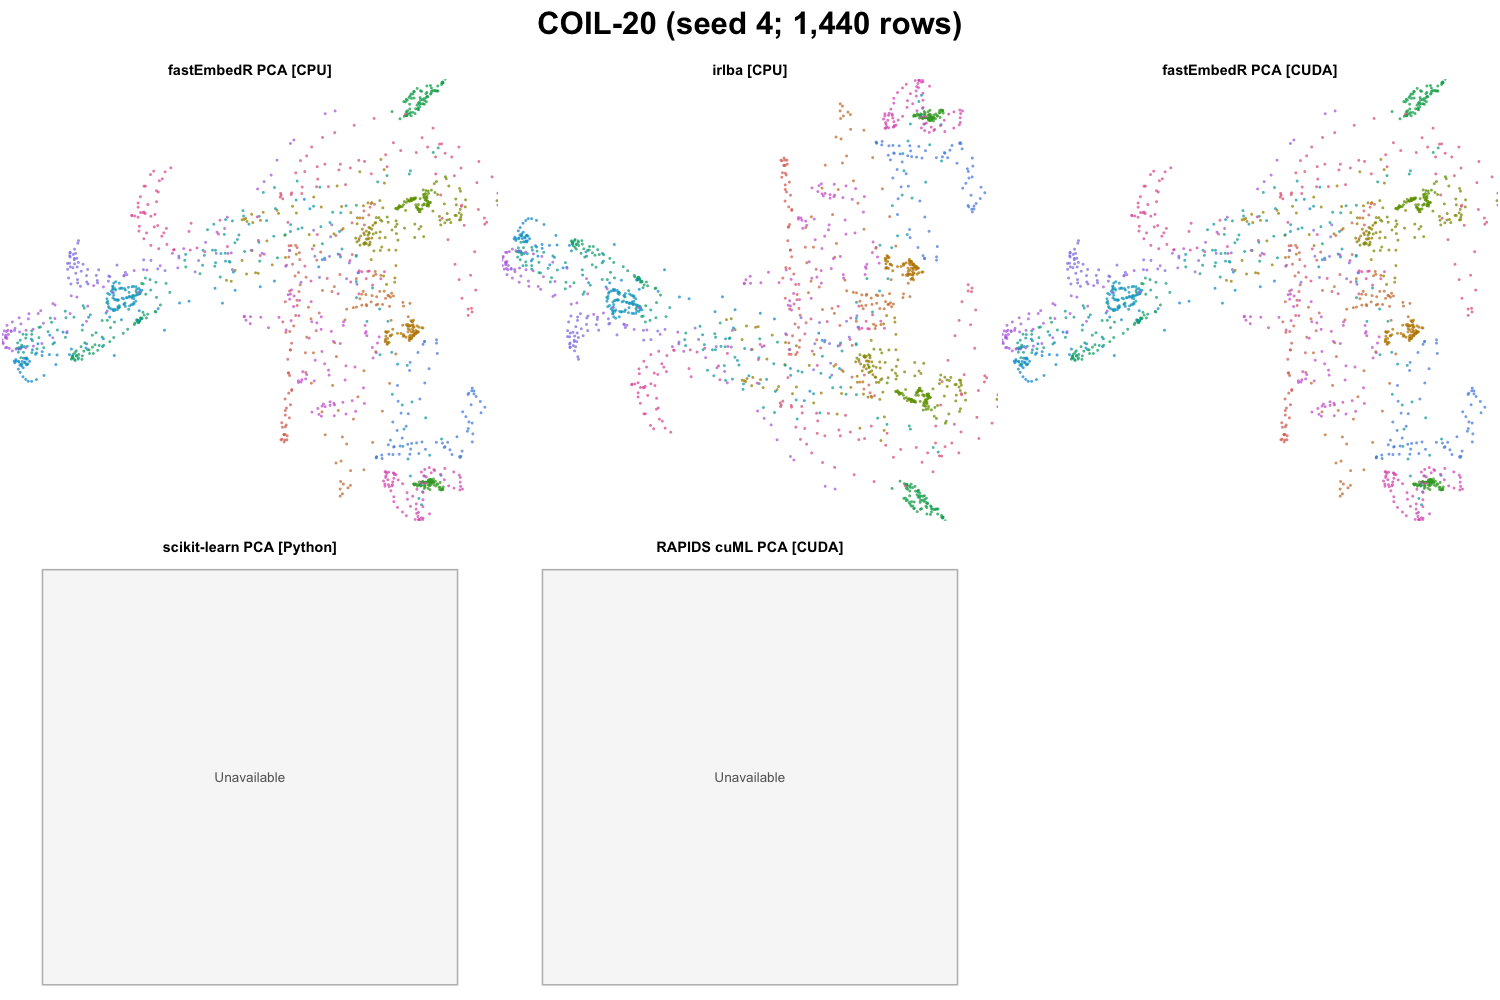
\includegraphics[width=0.94\textwidth]{figures/embedding_all_methods/COIL20_pca.png}
\caption{COIL-20 PCA outputs for the tested methods (seed 4; 1,440 rows). Colors encode benchmark labels and were not used for fitting.}
\end{figure}
\clearpage

\begin{figure}[p]
\centering
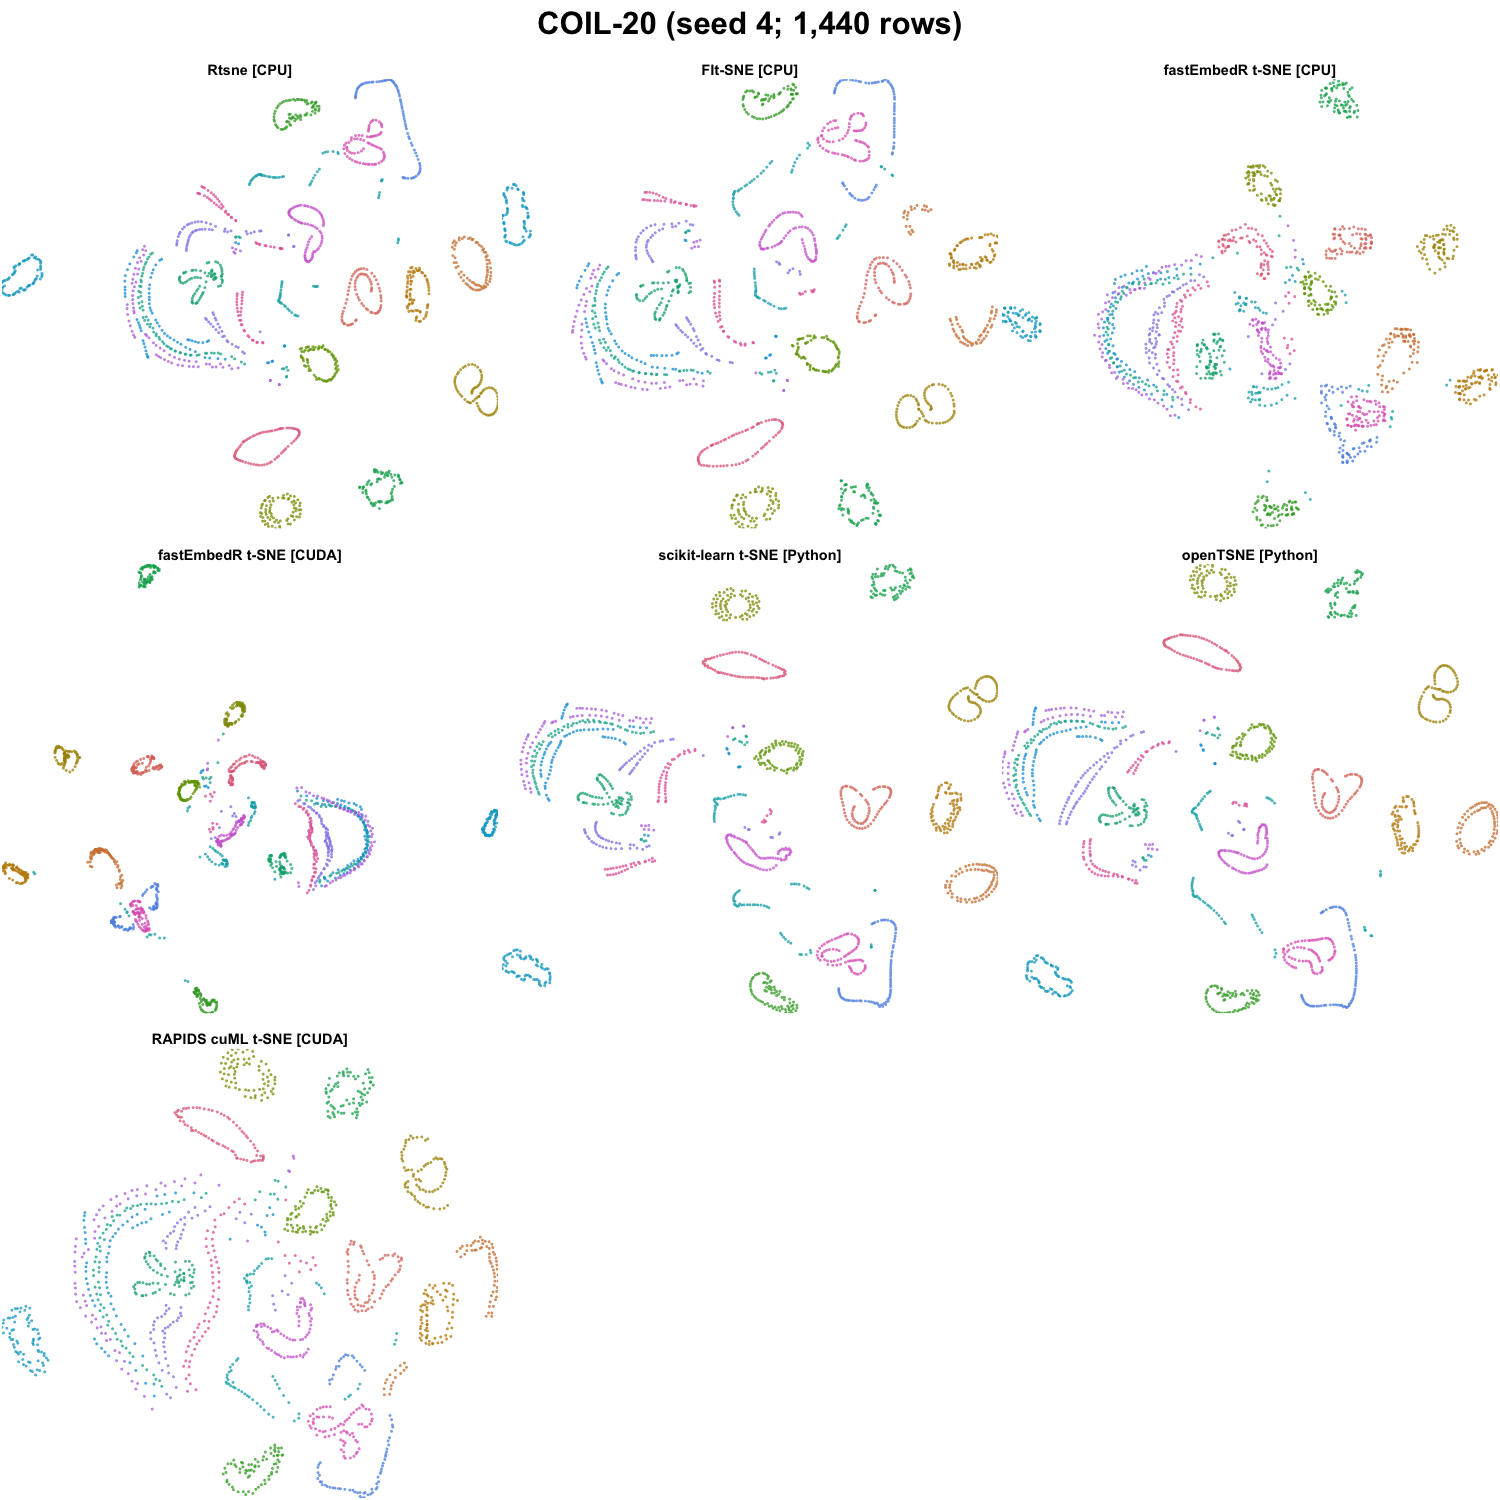
\includegraphics[width=0.94\textwidth]{figures/embedding_all_methods/COIL20_tsne.png}
\caption{COIL-20 t-SNE outputs for the tested methods (seed 4; 1,440 rows). Colors encode benchmark labels and were not used for fitting.}
\end{figure}
\clearpage

\begin{figure}[p]
\centering
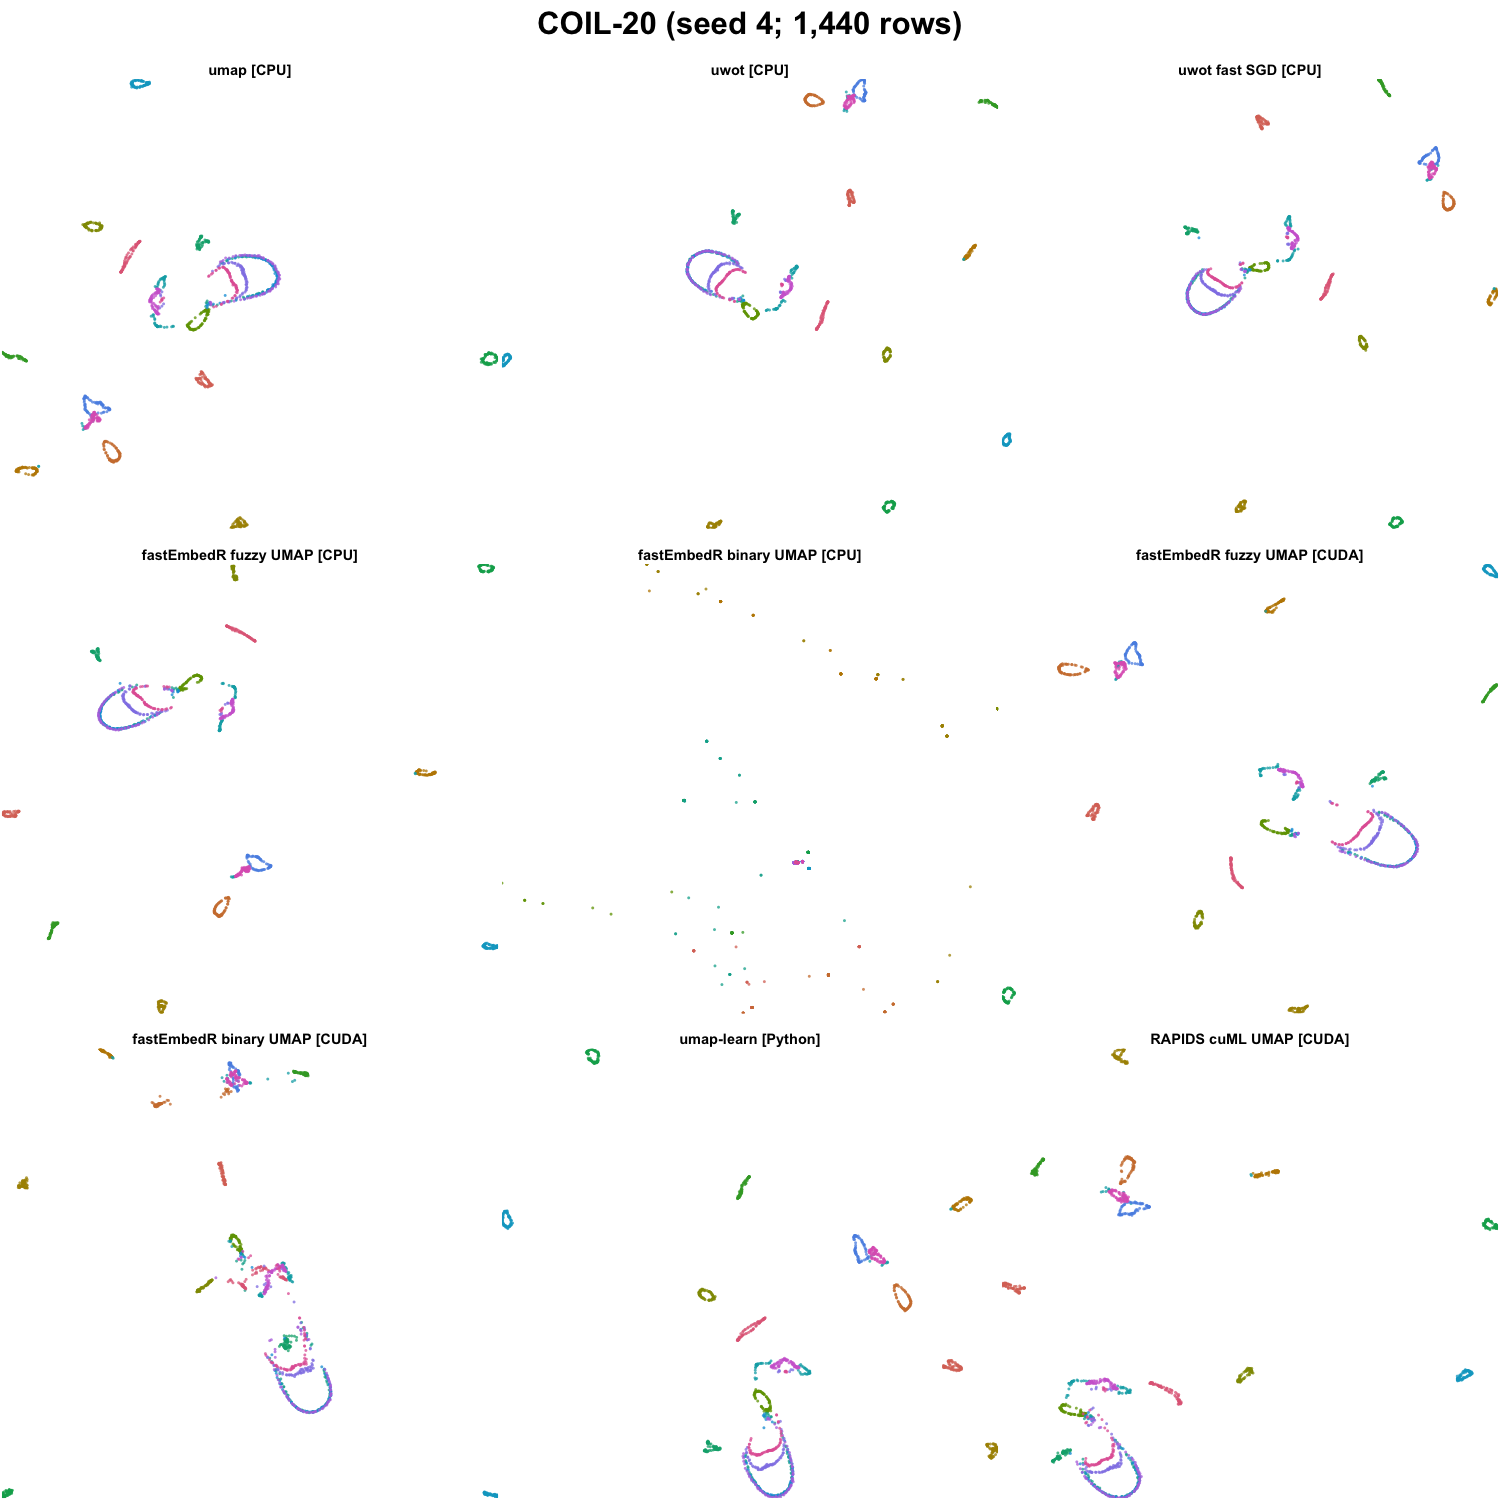
\includegraphics[width=0.94\textwidth]{figures/embedding_all_methods/COIL20_umap.png}
\caption{COIL-20 UMAP outputs for the tested methods (seed 4; 1,440 rows). Colors encode benchmark labels and were not used for fitting.}
\end{figure}
\clearpage

\begin{figure}[p]
\centering
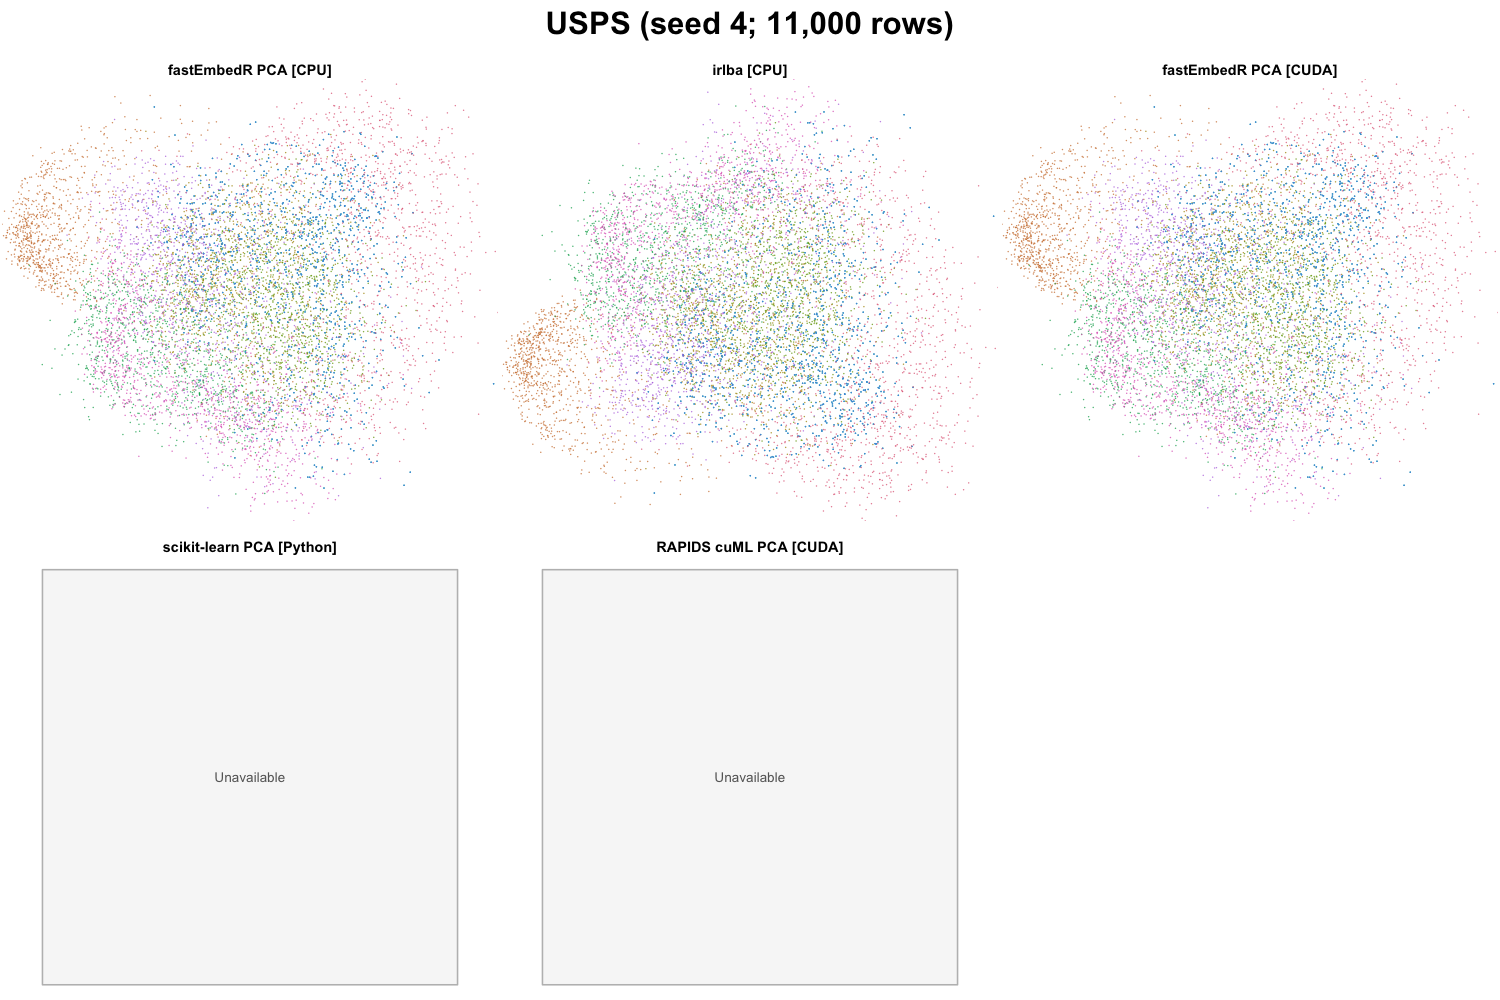
\includegraphics[width=0.94\textwidth]{figures/embedding_all_methods/USPS_pca.png}
\caption{USPS PCA outputs for the tested methods (seed 4; 11,000 rows). Colors encode benchmark labels and were not used for fitting.}
\end{figure}
\clearpage

\begin{figure}[p]
\centering
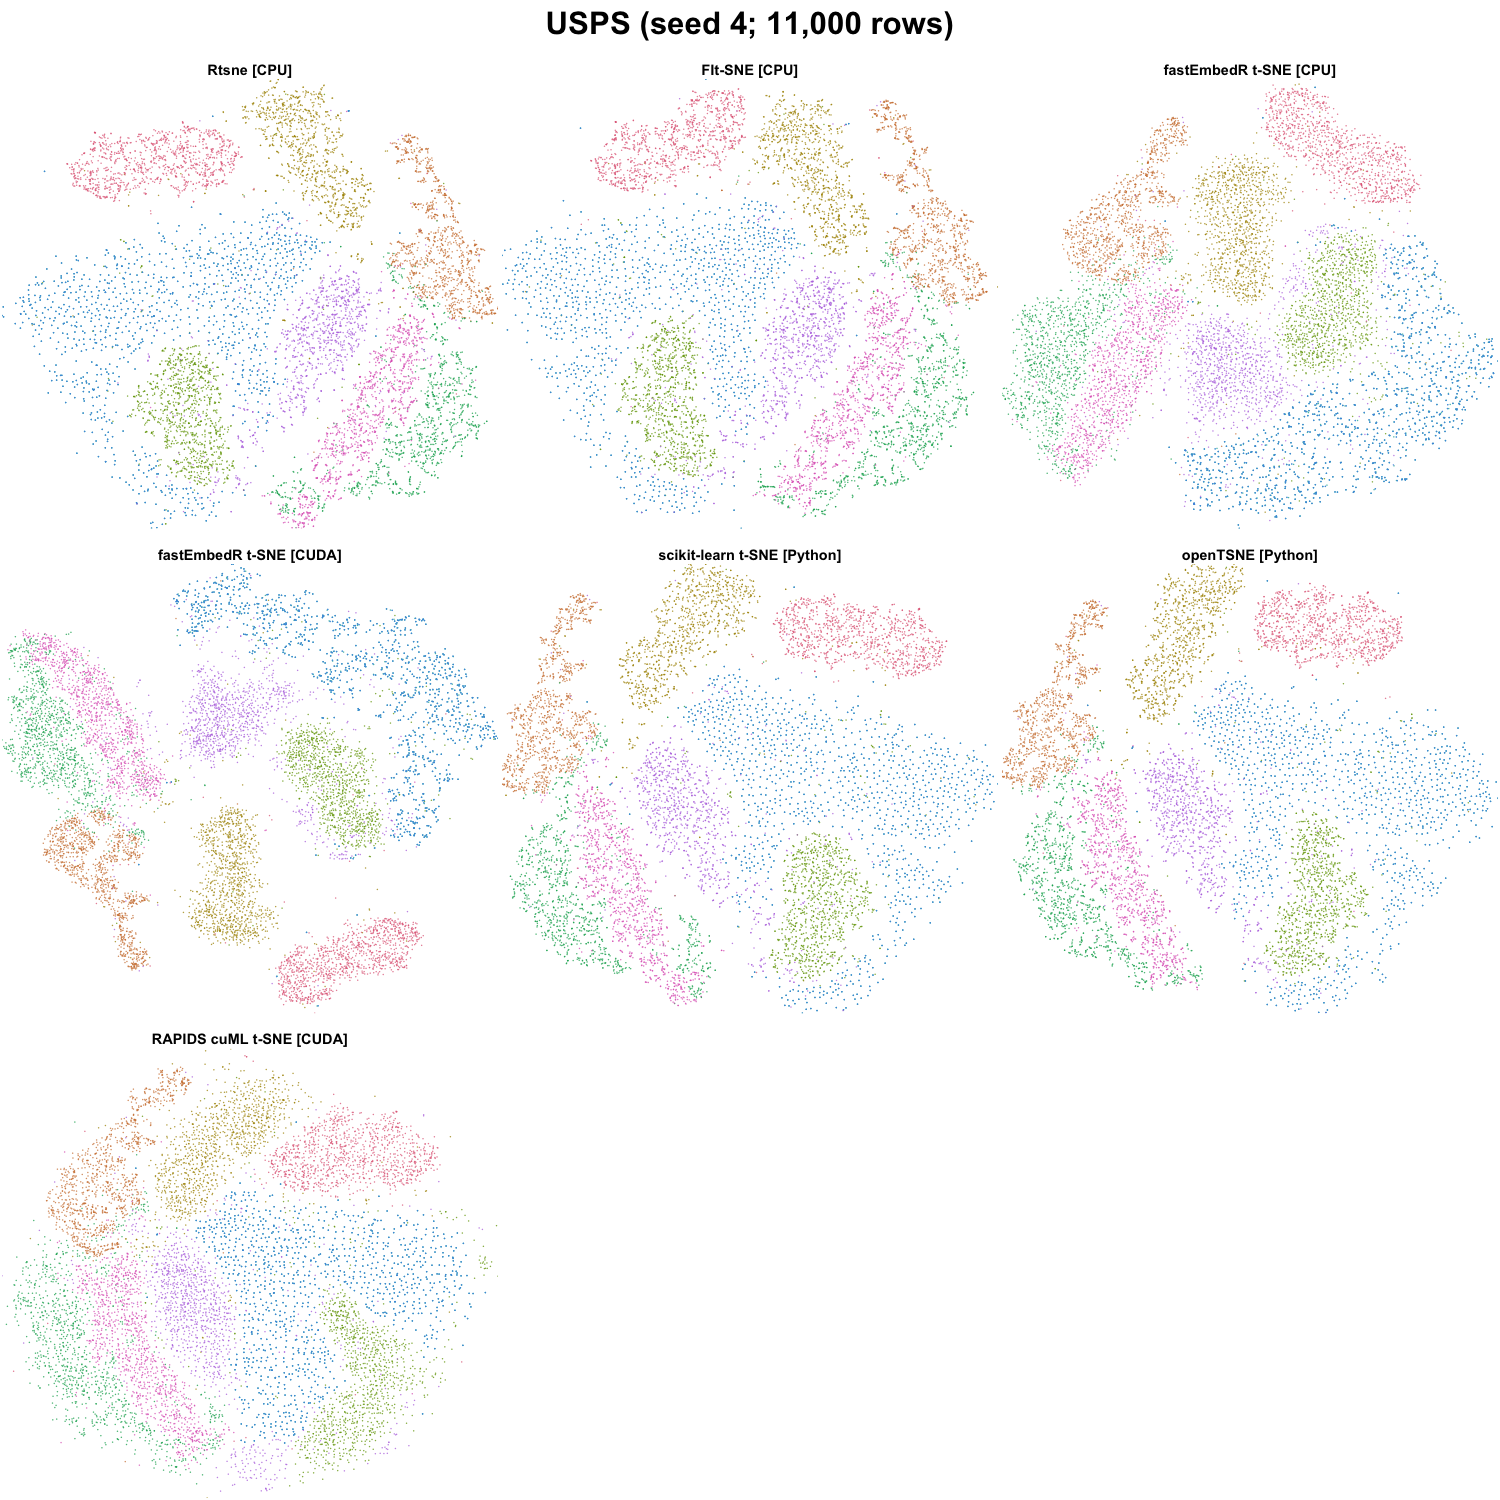
\includegraphics[width=0.94\textwidth]{figures/embedding_all_methods/USPS_tsne.png}
\caption{USPS t-SNE outputs for the tested methods (seed 4; 11,000 rows). Colors encode benchmark labels and were not used for fitting.}
\end{figure}
\clearpage

\begin{figure}[p]
\centering
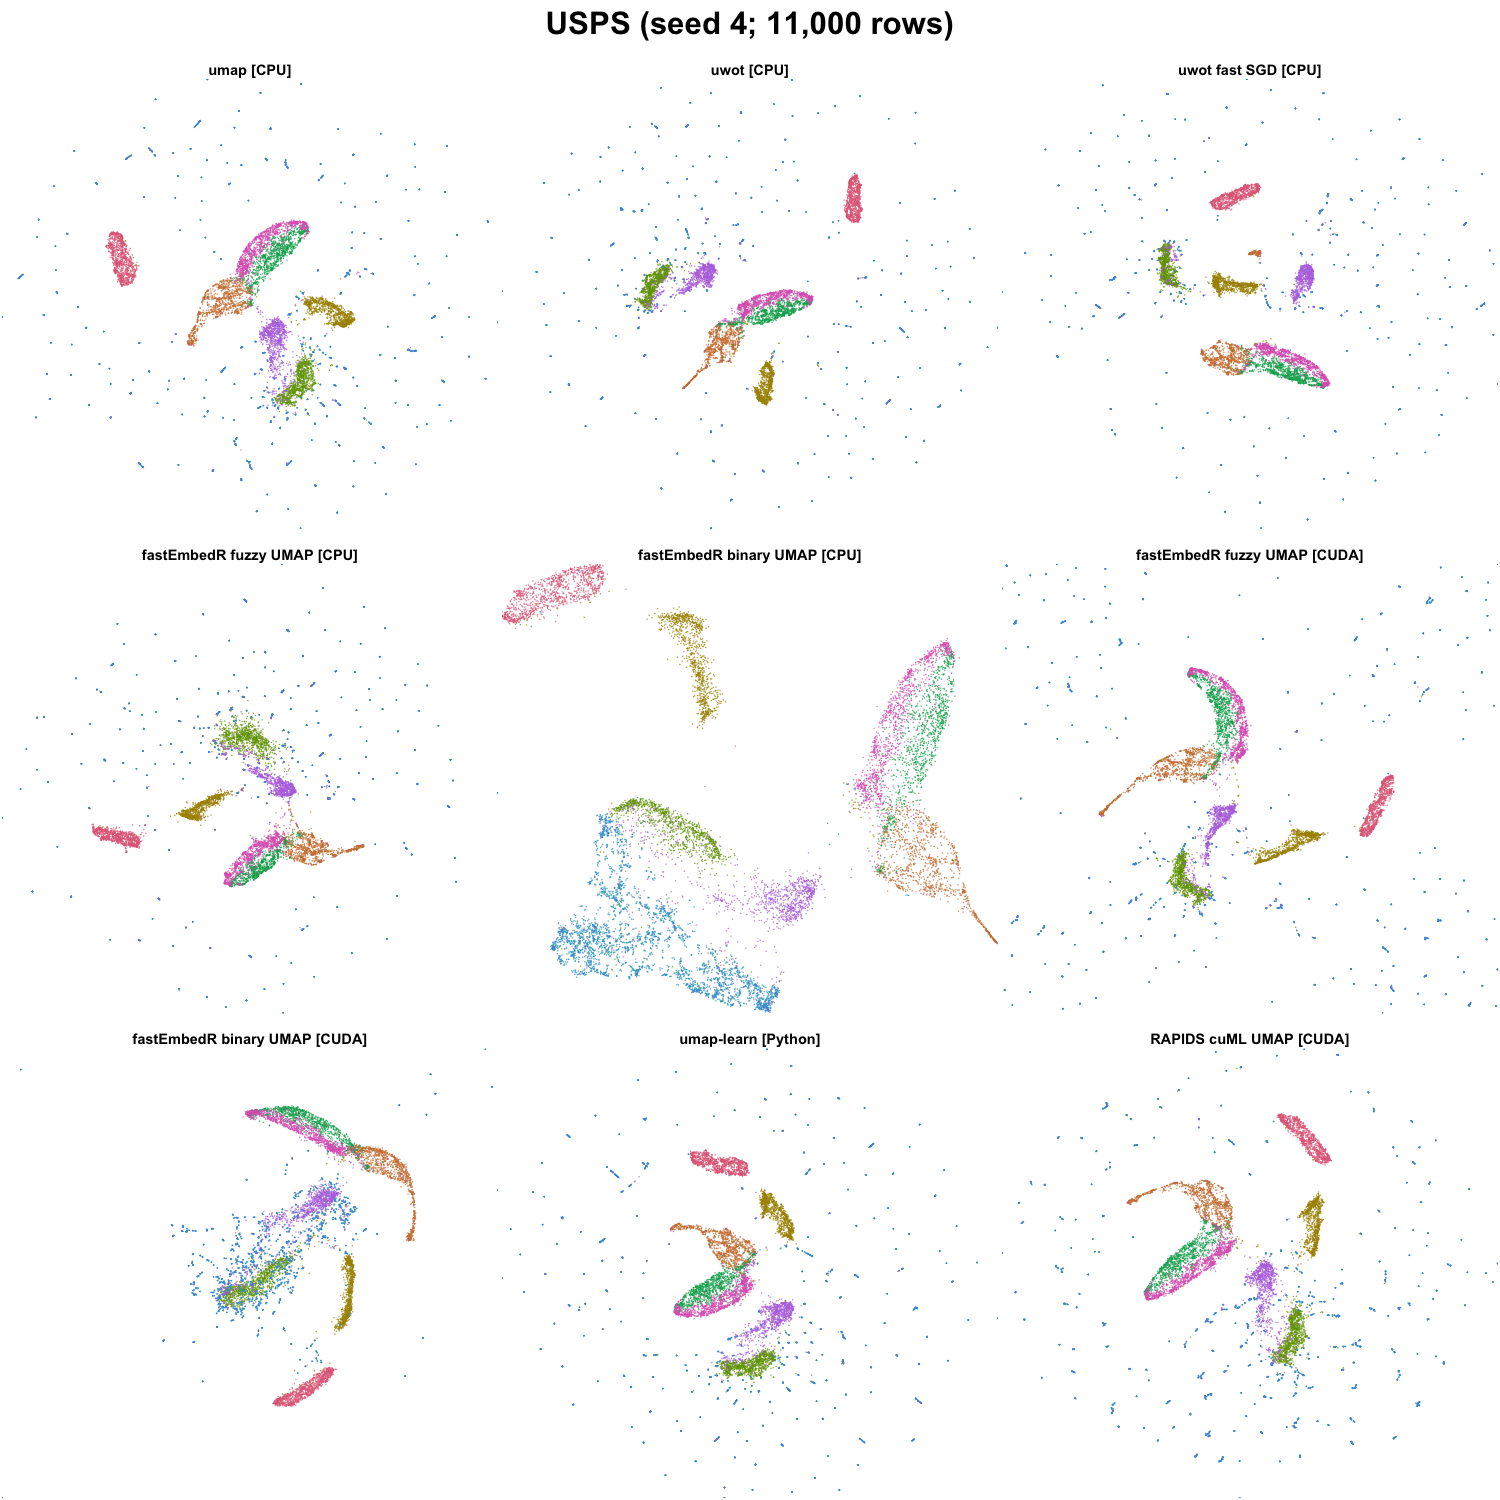
\includegraphics[width=0.94\textwidth]{figures/embedding_all_methods/USPS_umap.png}
\caption{USPS UMAP outputs for the tested methods (seed 4; 11,000 rows). Colors encode benchmark labels and were not used for fitting.}
\end{figure}
\clearpage

\begin{figure}[p]
\centering
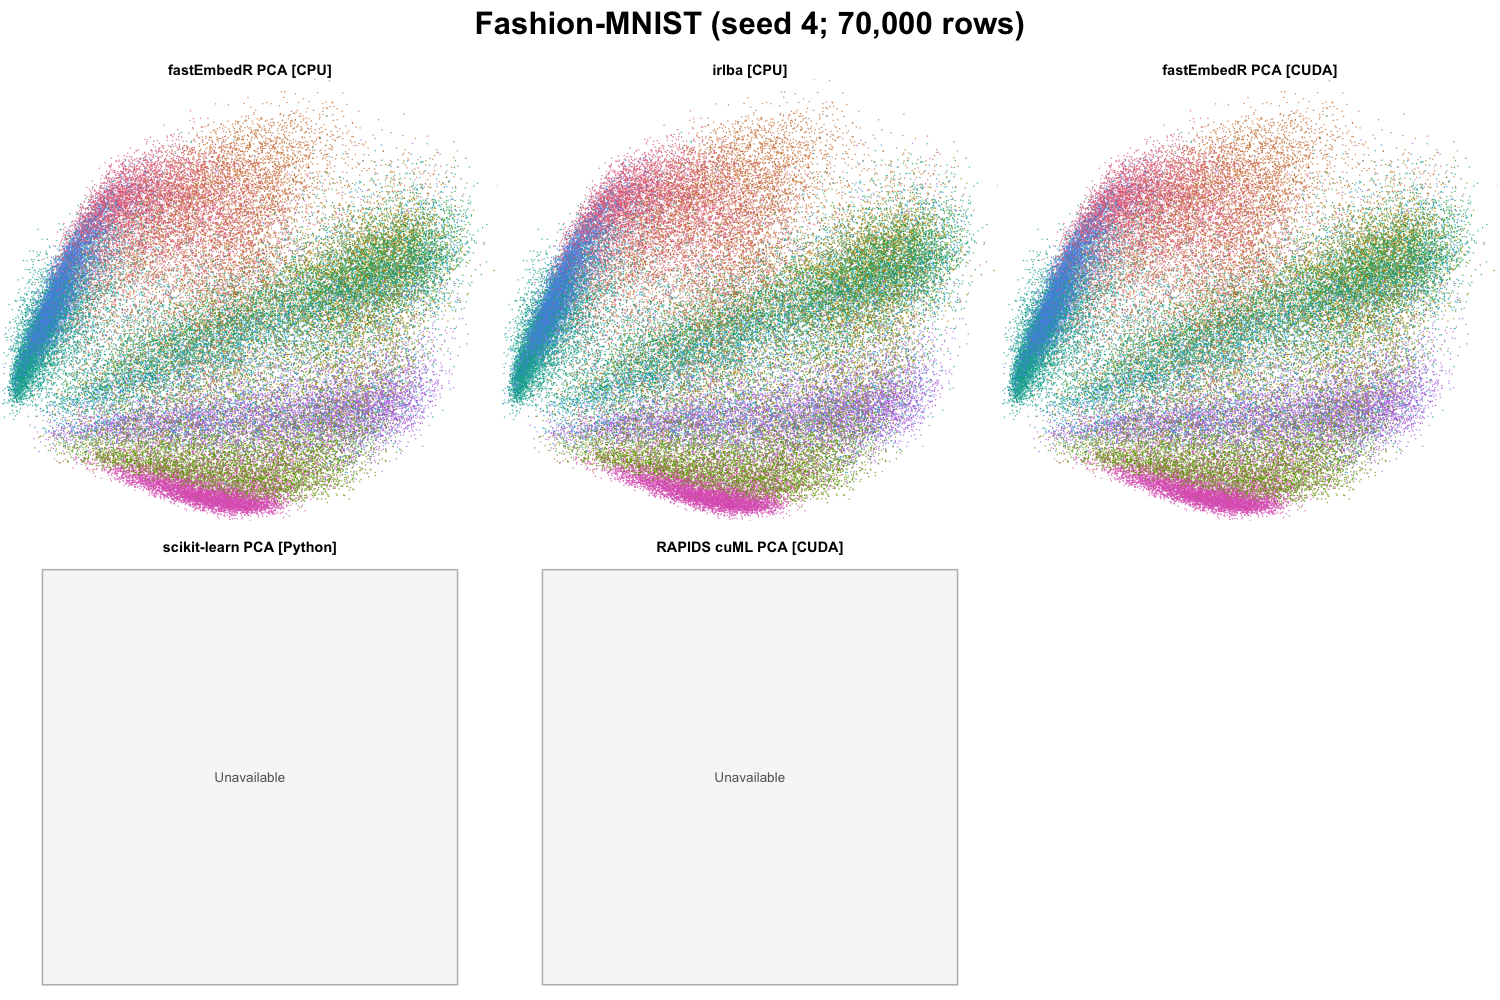
\includegraphics[width=0.94\textwidth]{figures/embedding_all_methods/FashionMNIST_pca.png}
\caption{Fashion-MNIST PCA outputs for the tested methods (seed 4; 70,000 rows). Colors encode benchmark labels and were not used for fitting.}
\end{figure}
\clearpage

\begin{figure}[p]
\centering
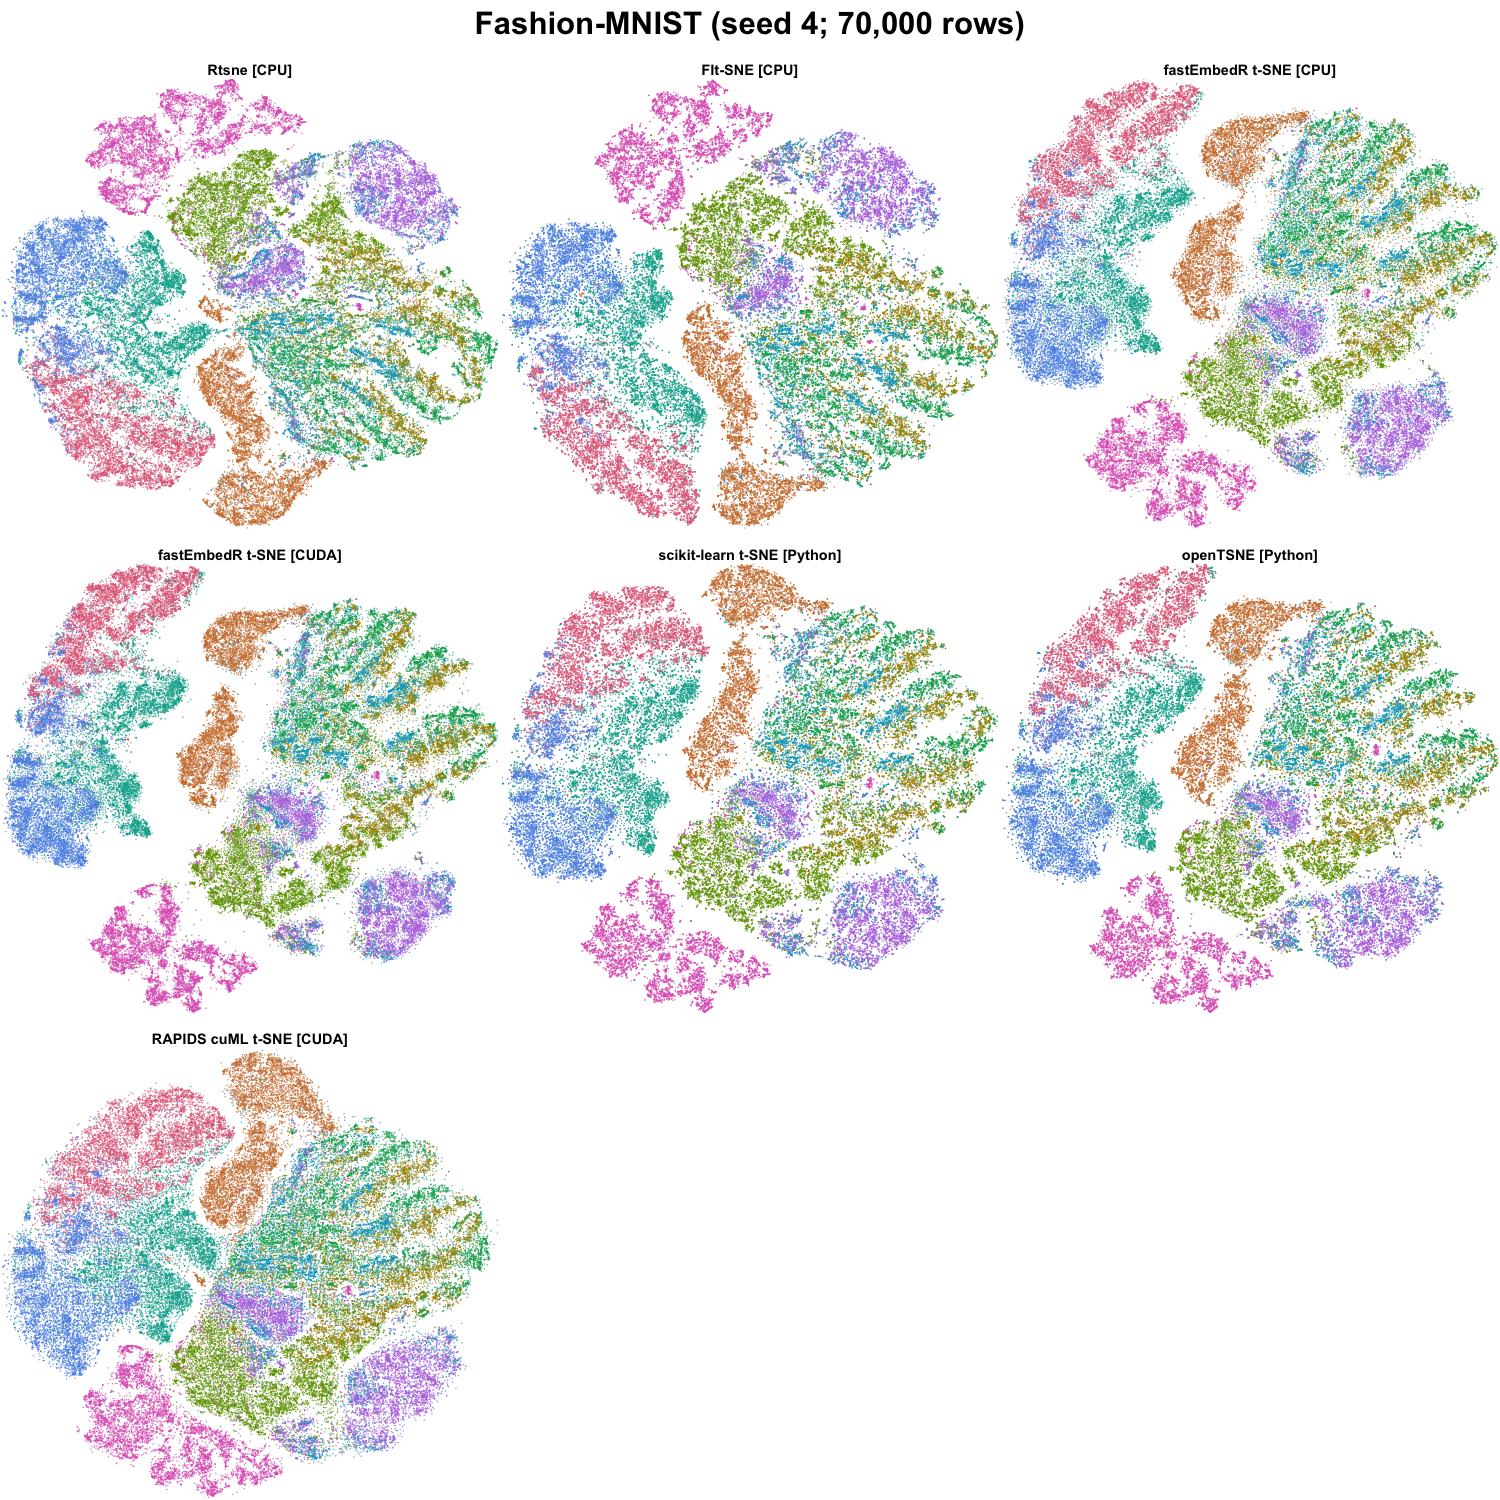
\includegraphics[width=0.94\textwidth]{figures/embedding_all_methods/FashionMNIST_tsne.png}
\caption{Fashion-MNIST t-SNE outputs for the tested methods (seed 4; 70,000 rows). Colors encode benchmark labels and were not used for fitting.}
\end{figure}
\clearpage

\begin{figure}[p]
\centering
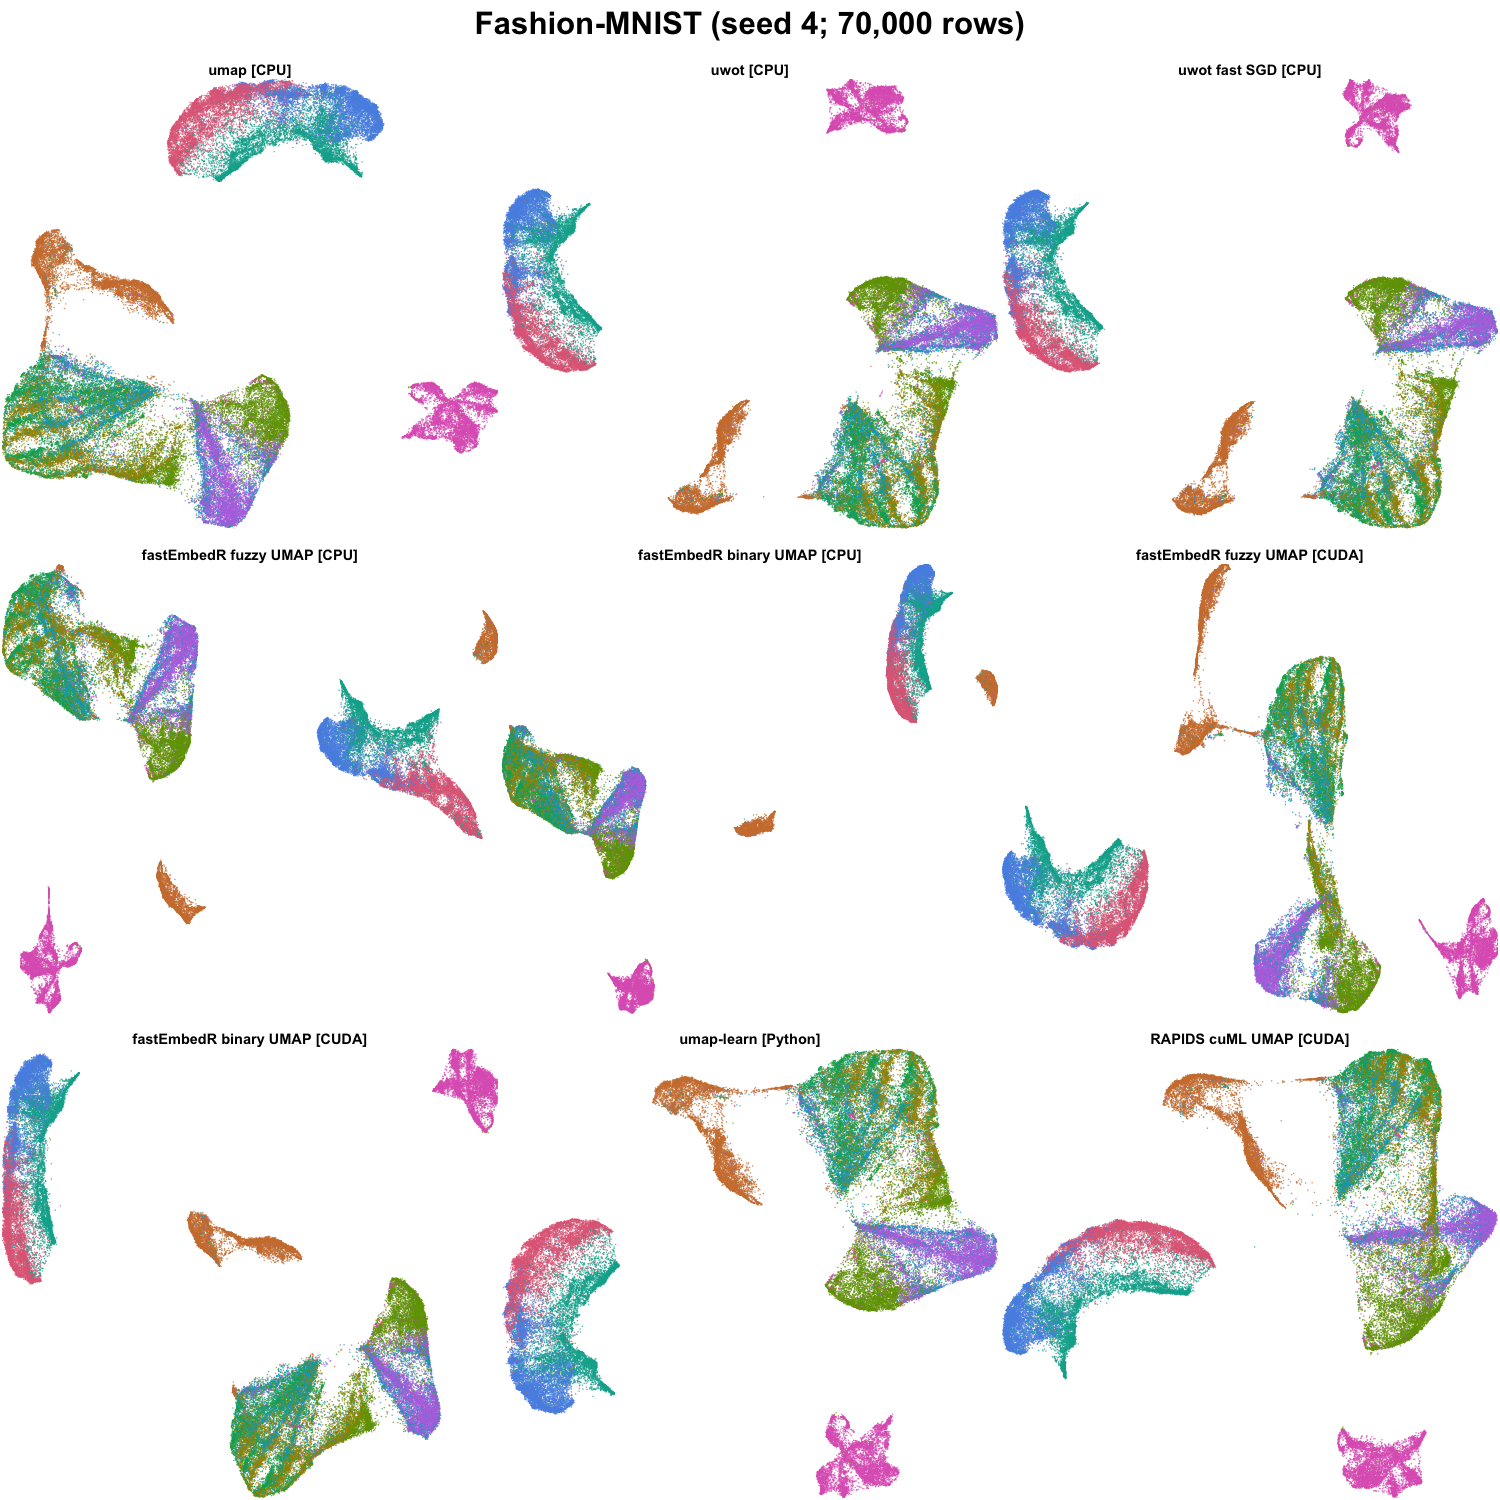
\includegraphics[width=0.94\textwidth]{figures/embedding_all_methods/FashionMNIST_umap.png}
\caption{Fashion-MNIST UMAP outputs for the tested methods (seed 4; 70,000 rows). Colors encode benchmark labels and were not used for fitting.}
\end{figure}
\clearpage

\begin{figure}[p]
\centering
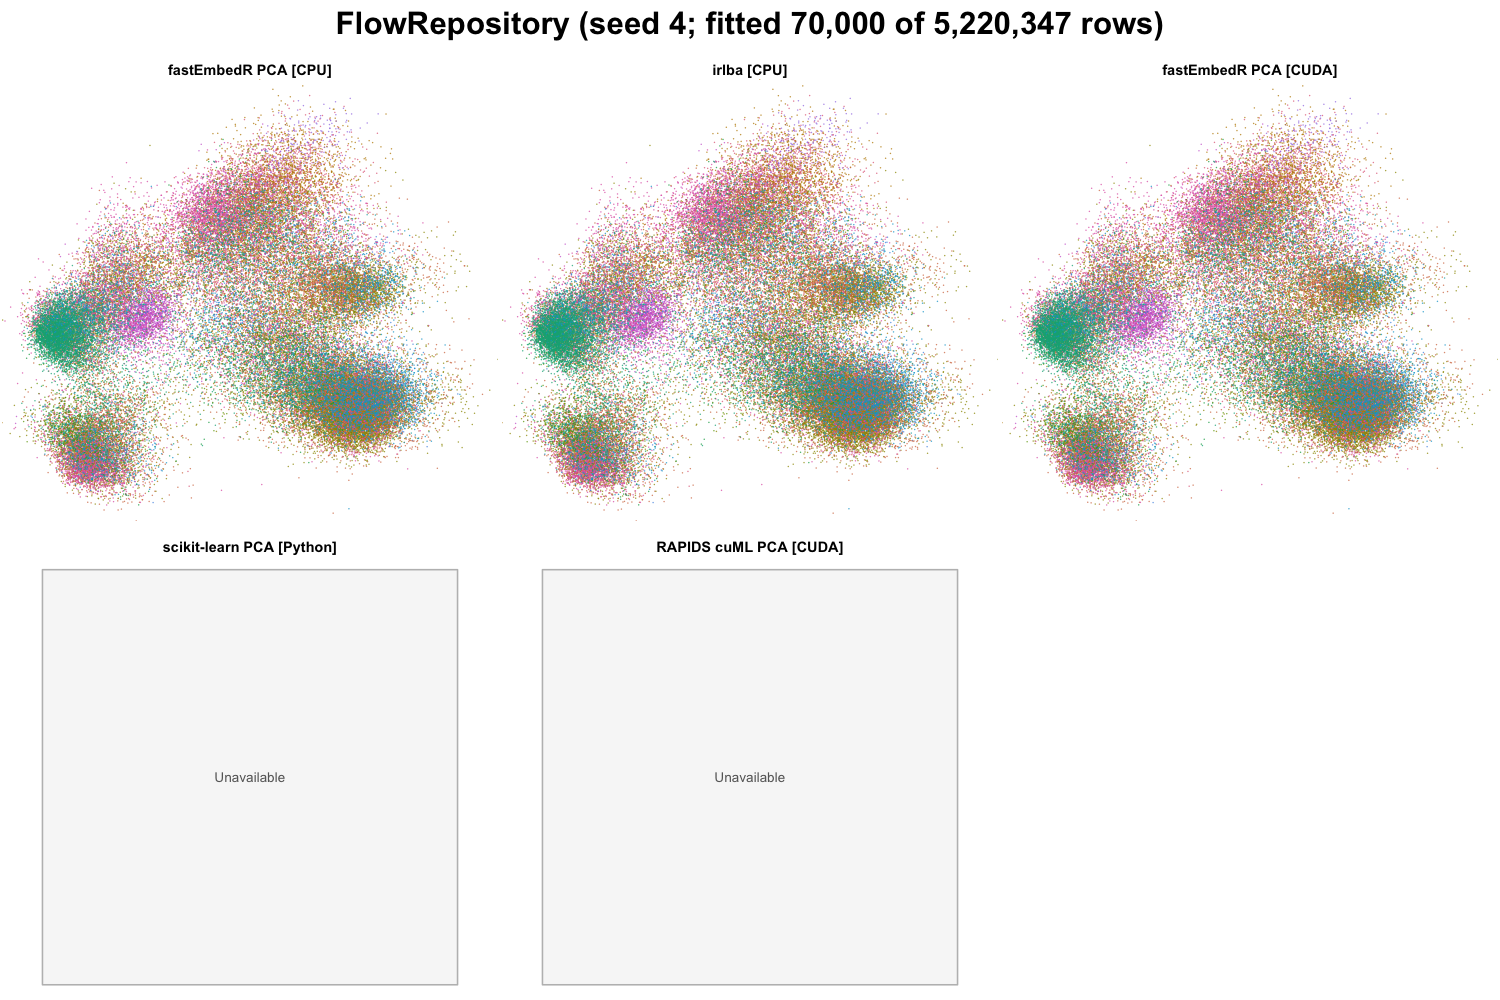
\includegraphics[width=0.94\textwidth]{figures/embedding_all_methods/FlowRepository_FR_FCM_ZYRM_files_pca.png}
\caption{FlowRepository PCA outputs for the tested methods (seed 4; fitted 70,000 of 5,220,347 rows). Colors encode benchmark labels and were not used for fitting.}
\end{figure}
\clearpage

\begin{figure}[p]
\centering
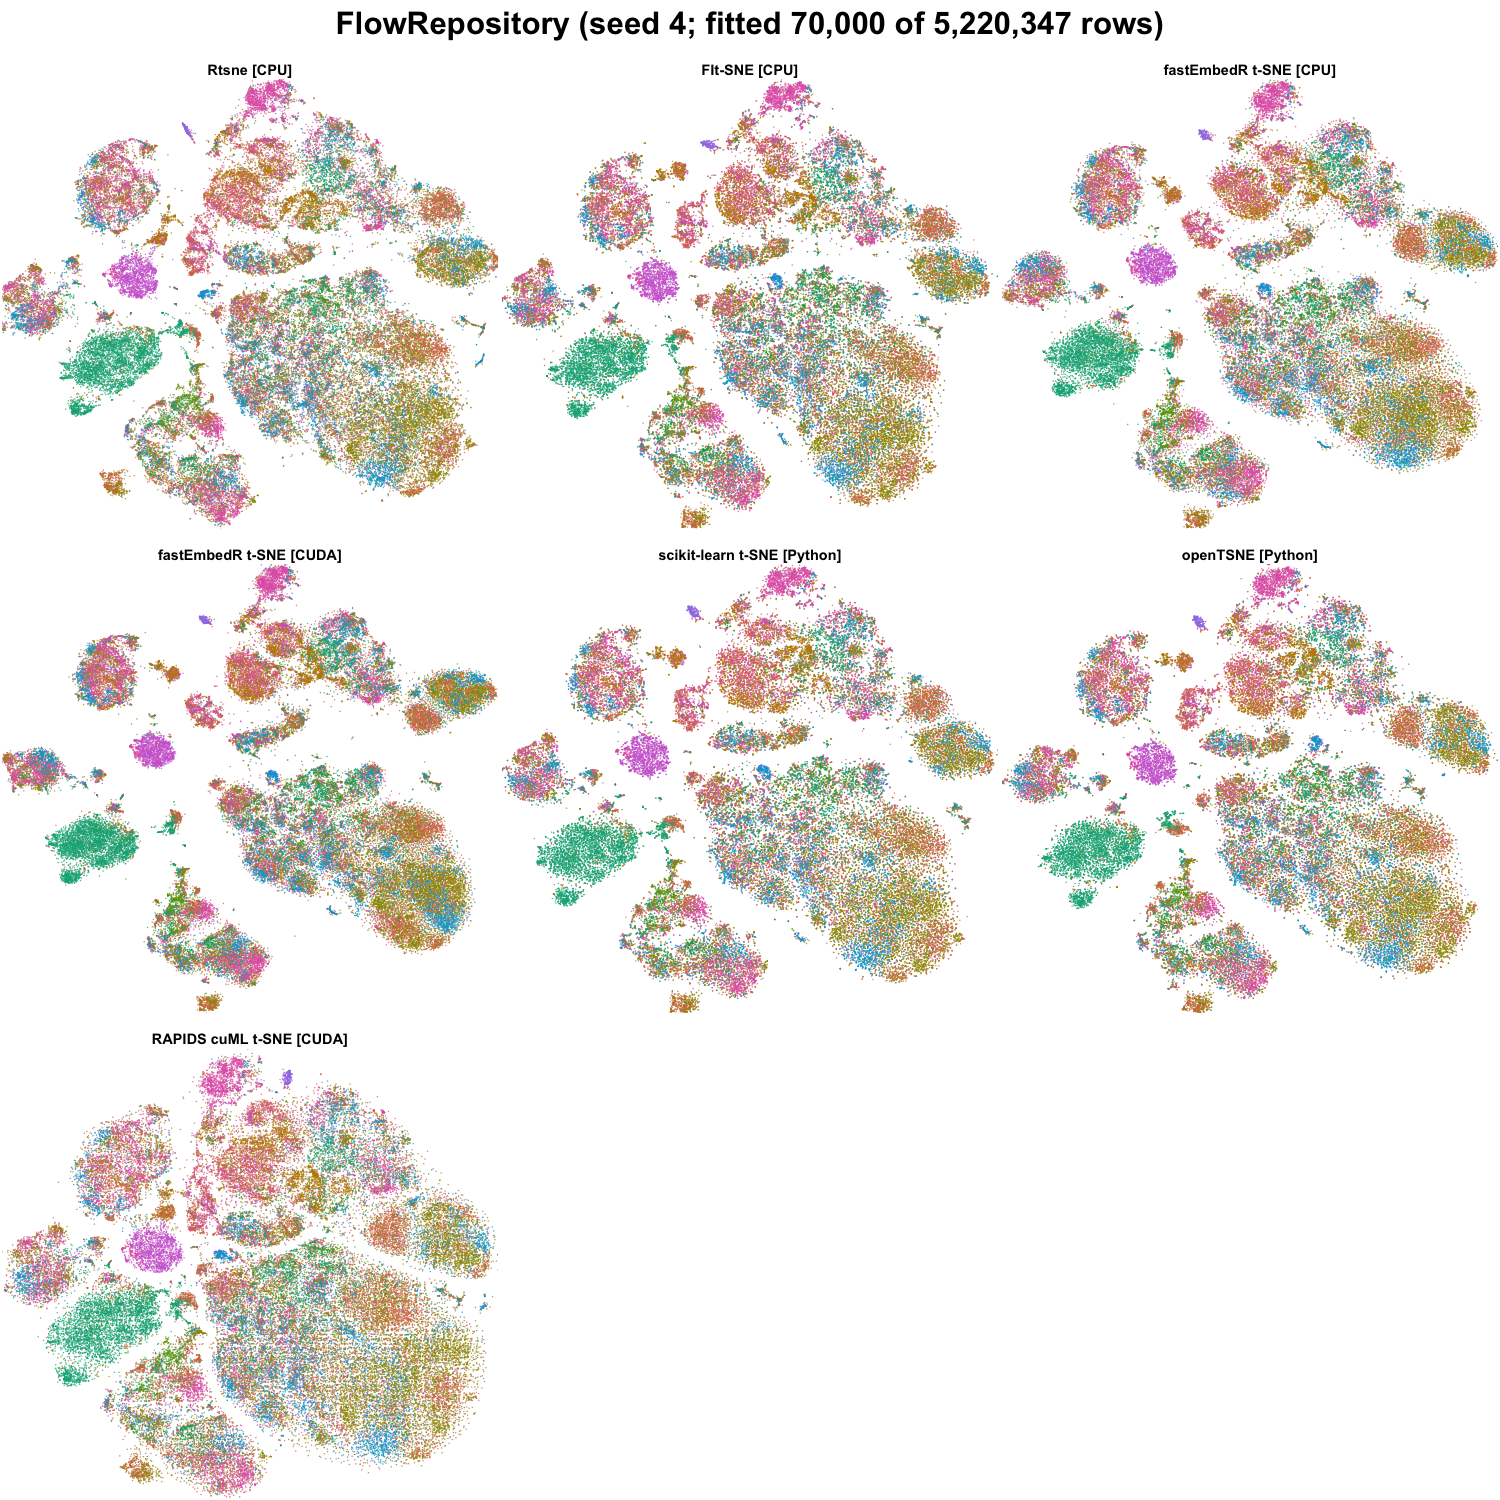
\includegraphics[width=0.94\textwidth]{figures/embedding_all_methods/FlowRepository_FR_FCM_ZYRM_files_tsne.png}
\caption{FlowRepository t-SNE outputs for the tested methods (seed 4; fitted 70,000 of 5,220,347 rows). Colors encode benchmark labels and were not used for fitting.}
\end{figure}
\clearpage

\begin{figure}[p]
\centering
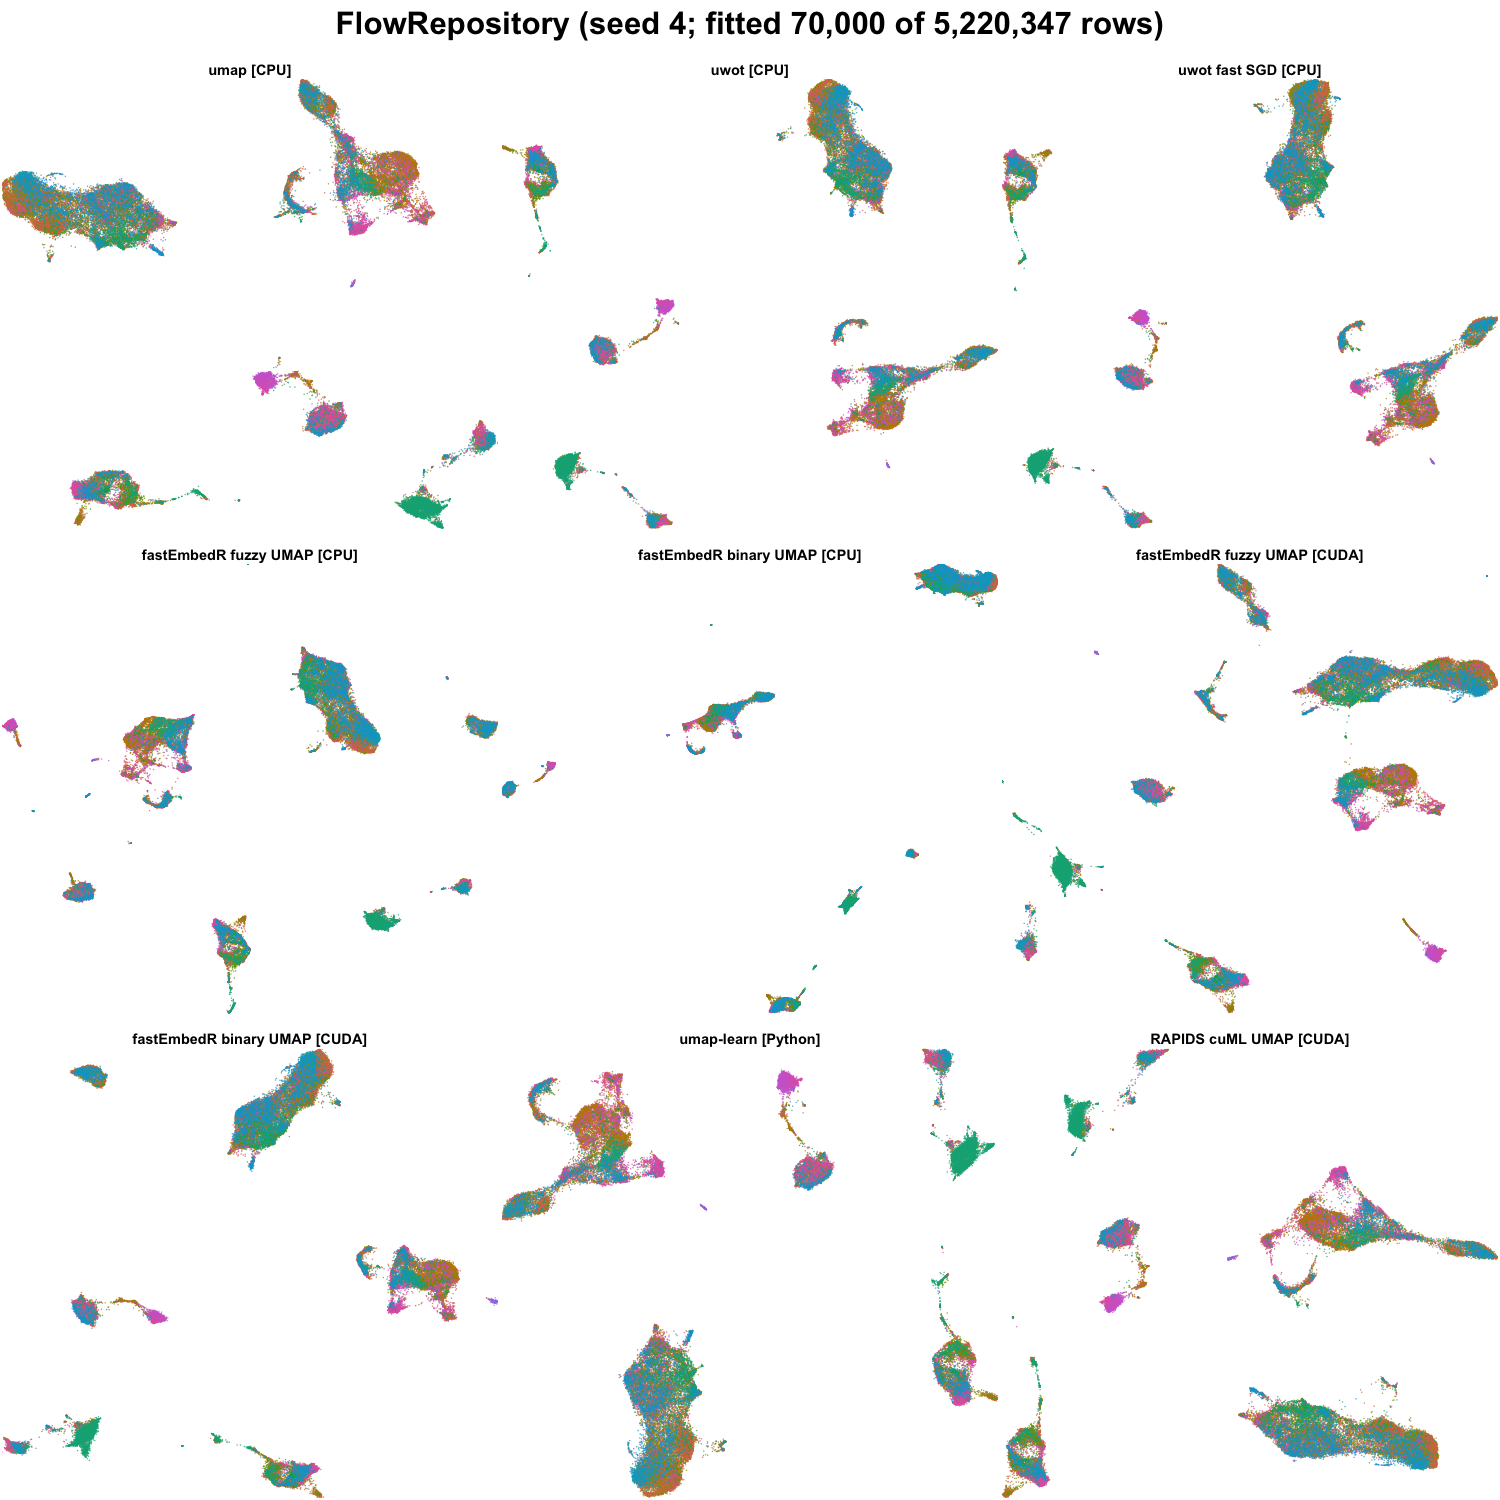
\includegraphics[width=0.94\textwidth]{figures/embedding_all_methods/FlowRepository_FR_FCM_ZYRM_files_umap.png}
\caption{FlowRepository UMAP outputs for the tested methods (seed 4; fitted 70,000 of 5,220,347 rows). Colors encode benchmark labels and were not used for fitting.}
\end{figure}
\clearpage

\begin{figure}[p]
\centering
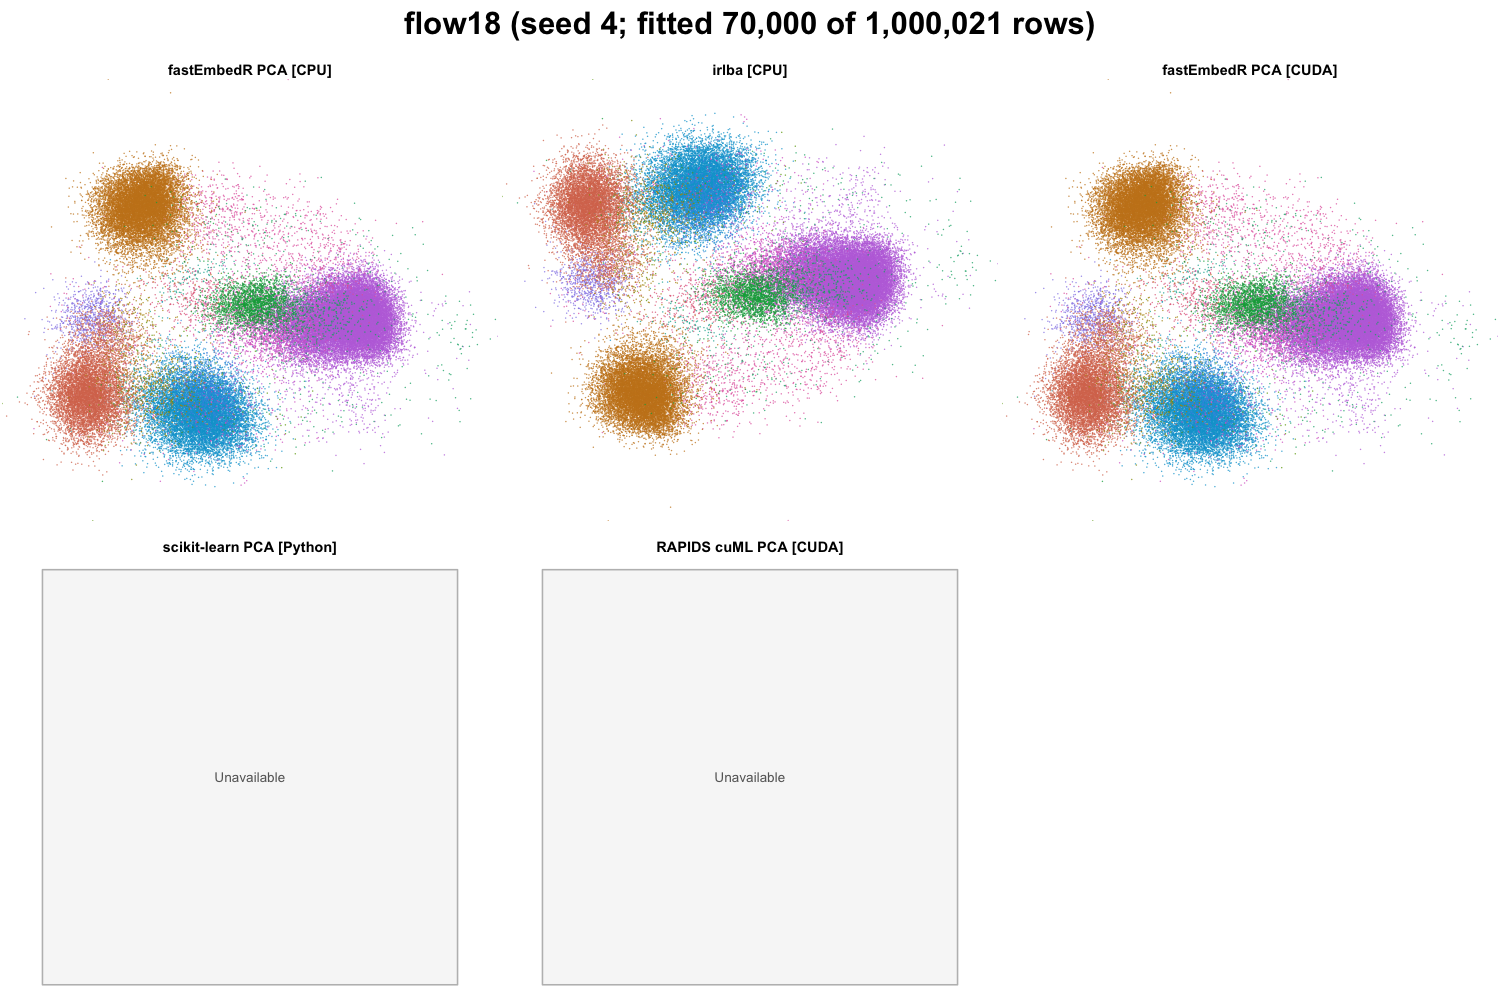
\includegraphics[width=0.94\textwidth]{figures/embedding_all_methods/flow18_pca.png}
\caption{flow18 PCA outputs for the tested methods (seed 4; fitted 70,000 of 1,000,021 rows). Colors encode benchmark labels and were not used for fitting.}
\end{figure}
\clearpage

\begin{figure}[p]
\centering
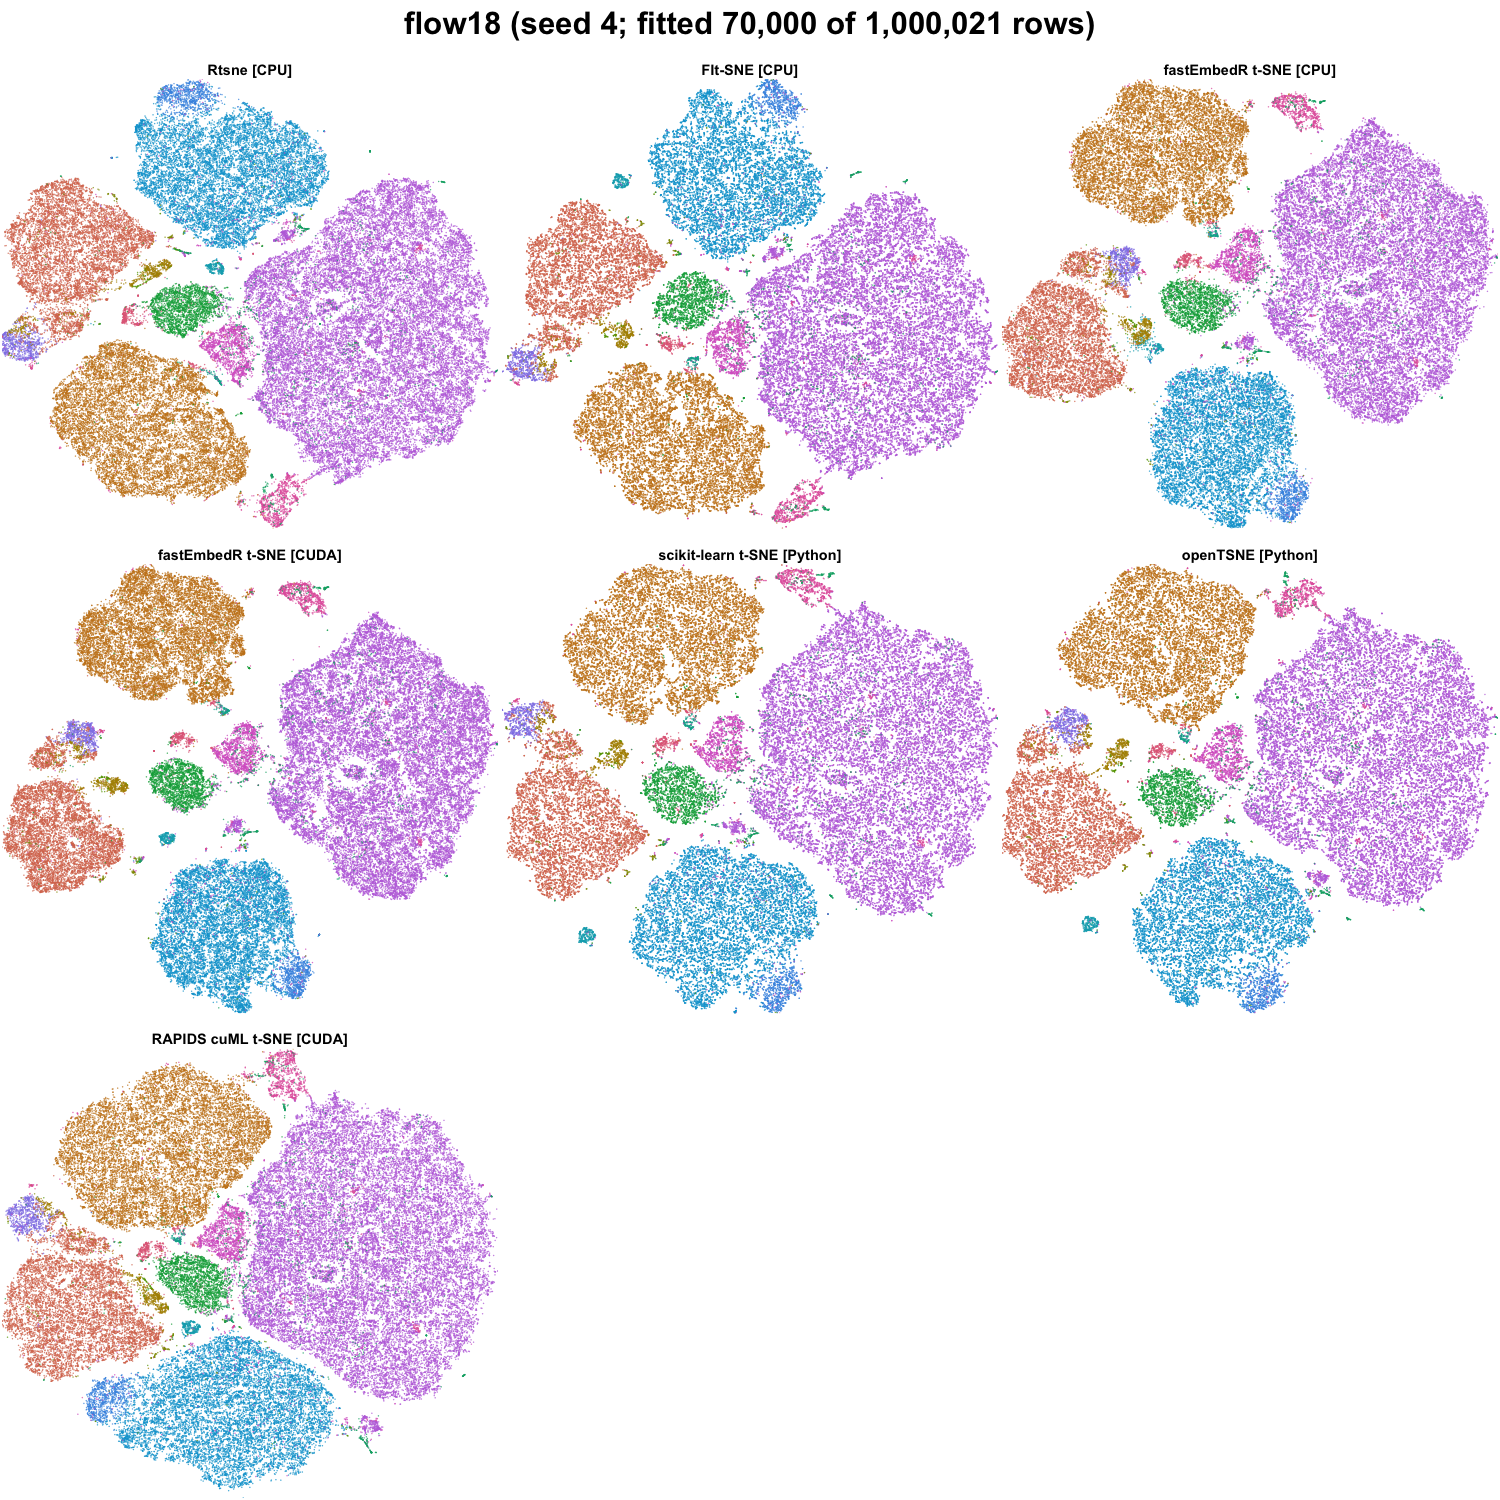
\includegraphics[width=0.94\textwidth]{figures/embedding_all_methods/flow18_tsne.png}
\caption{flow18 t-SNE outputs for the tested methods (seed 4; fitted 70,000 of 1,000,021 rows). Colors encode benchmark labels and were not used for fitting.}
\end{figure}
\clearpage

\begin{figure}[p]
\centering
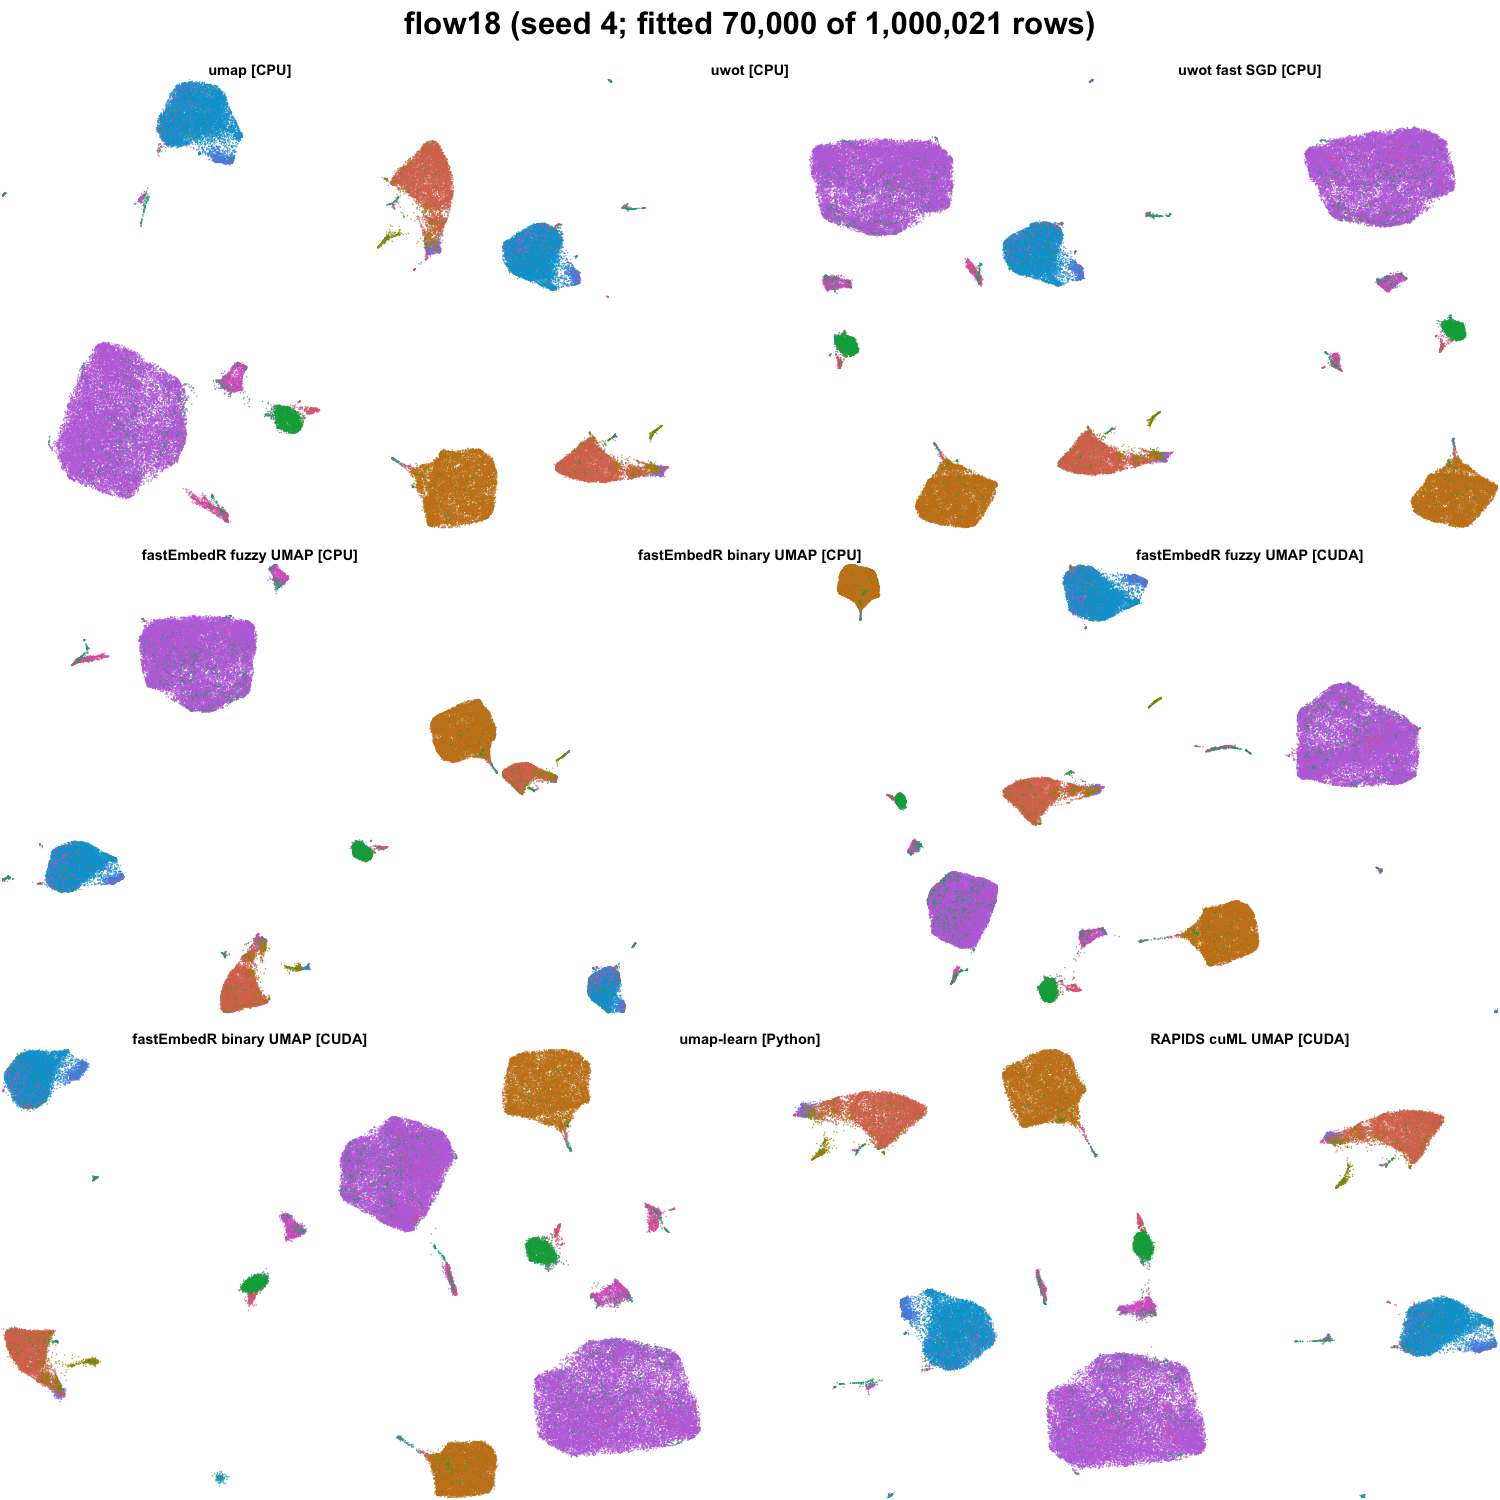
\includegraphics[width=0.94\textwidth]{figures/embedding_all_methods/flow18_umap.png}
\caption{flow18 UMAP outputs for the tested methods (seed 4; fitted 70,000 of 1,000,021 rows). Colors encode benchmark labels and were not used for fitting.}
\end{figure}
\clearpage

\begin{figure}[p]
\centering
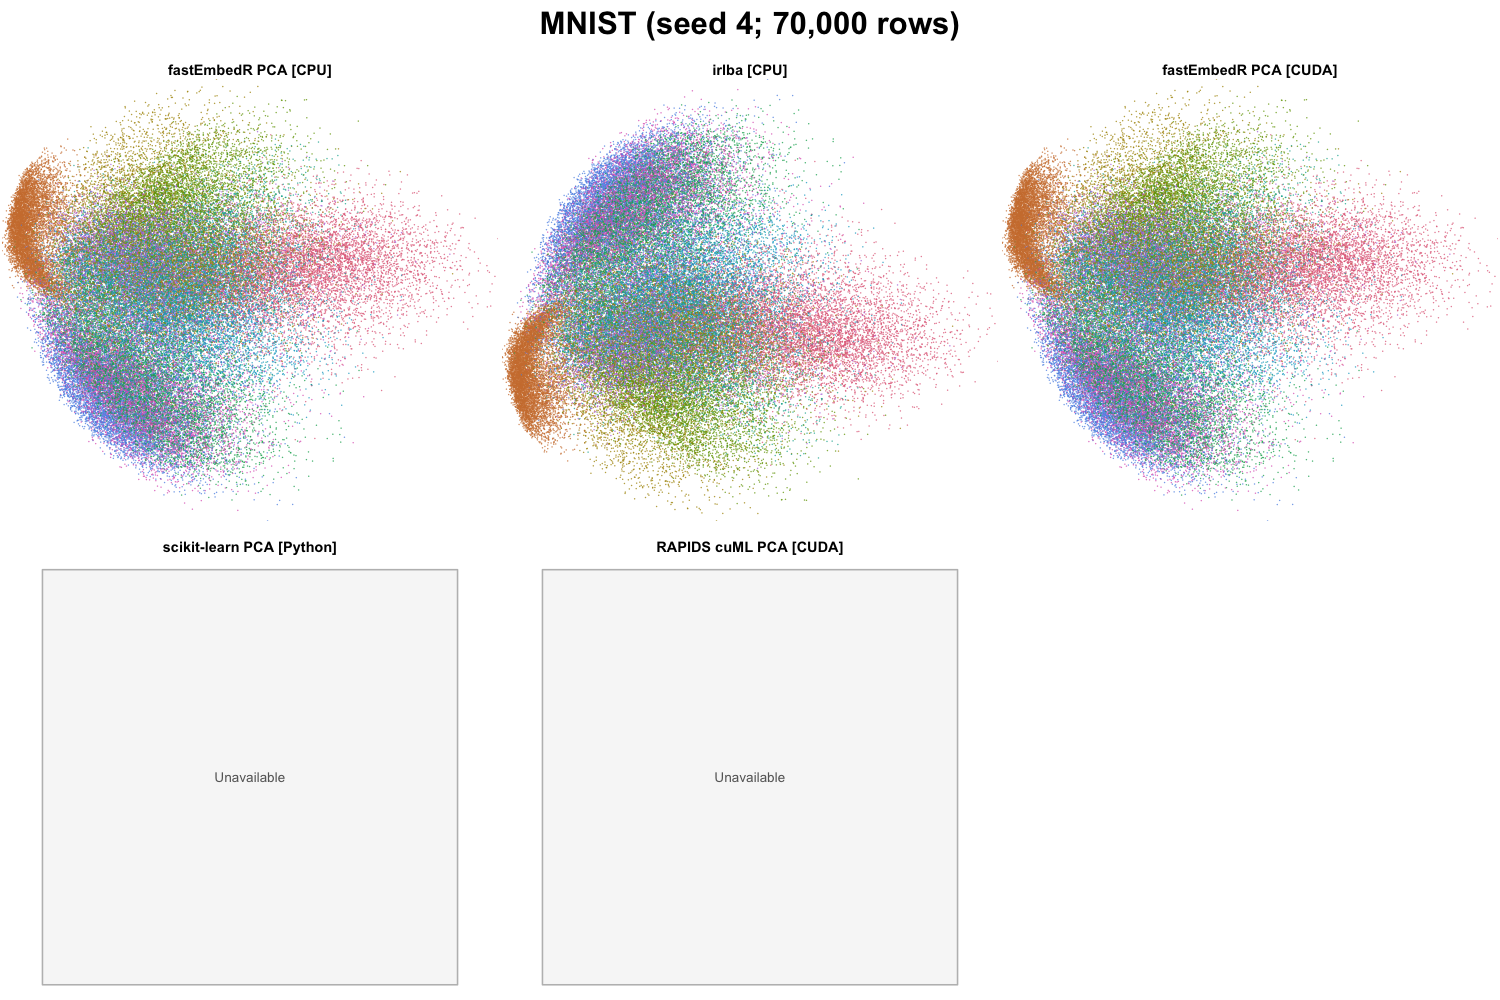
\includegraphics[width=0.94\textwidth]{figures/embedding_all_methods/MNIST_pca.png}
\caption{MNIST PCA outputs for the tested methods (seed 4; 70,000 rows). Colors encode benchmark labels and were not used for fitting.}
\end{figure}
\clearpage

\begin{figure}[p]
\centering
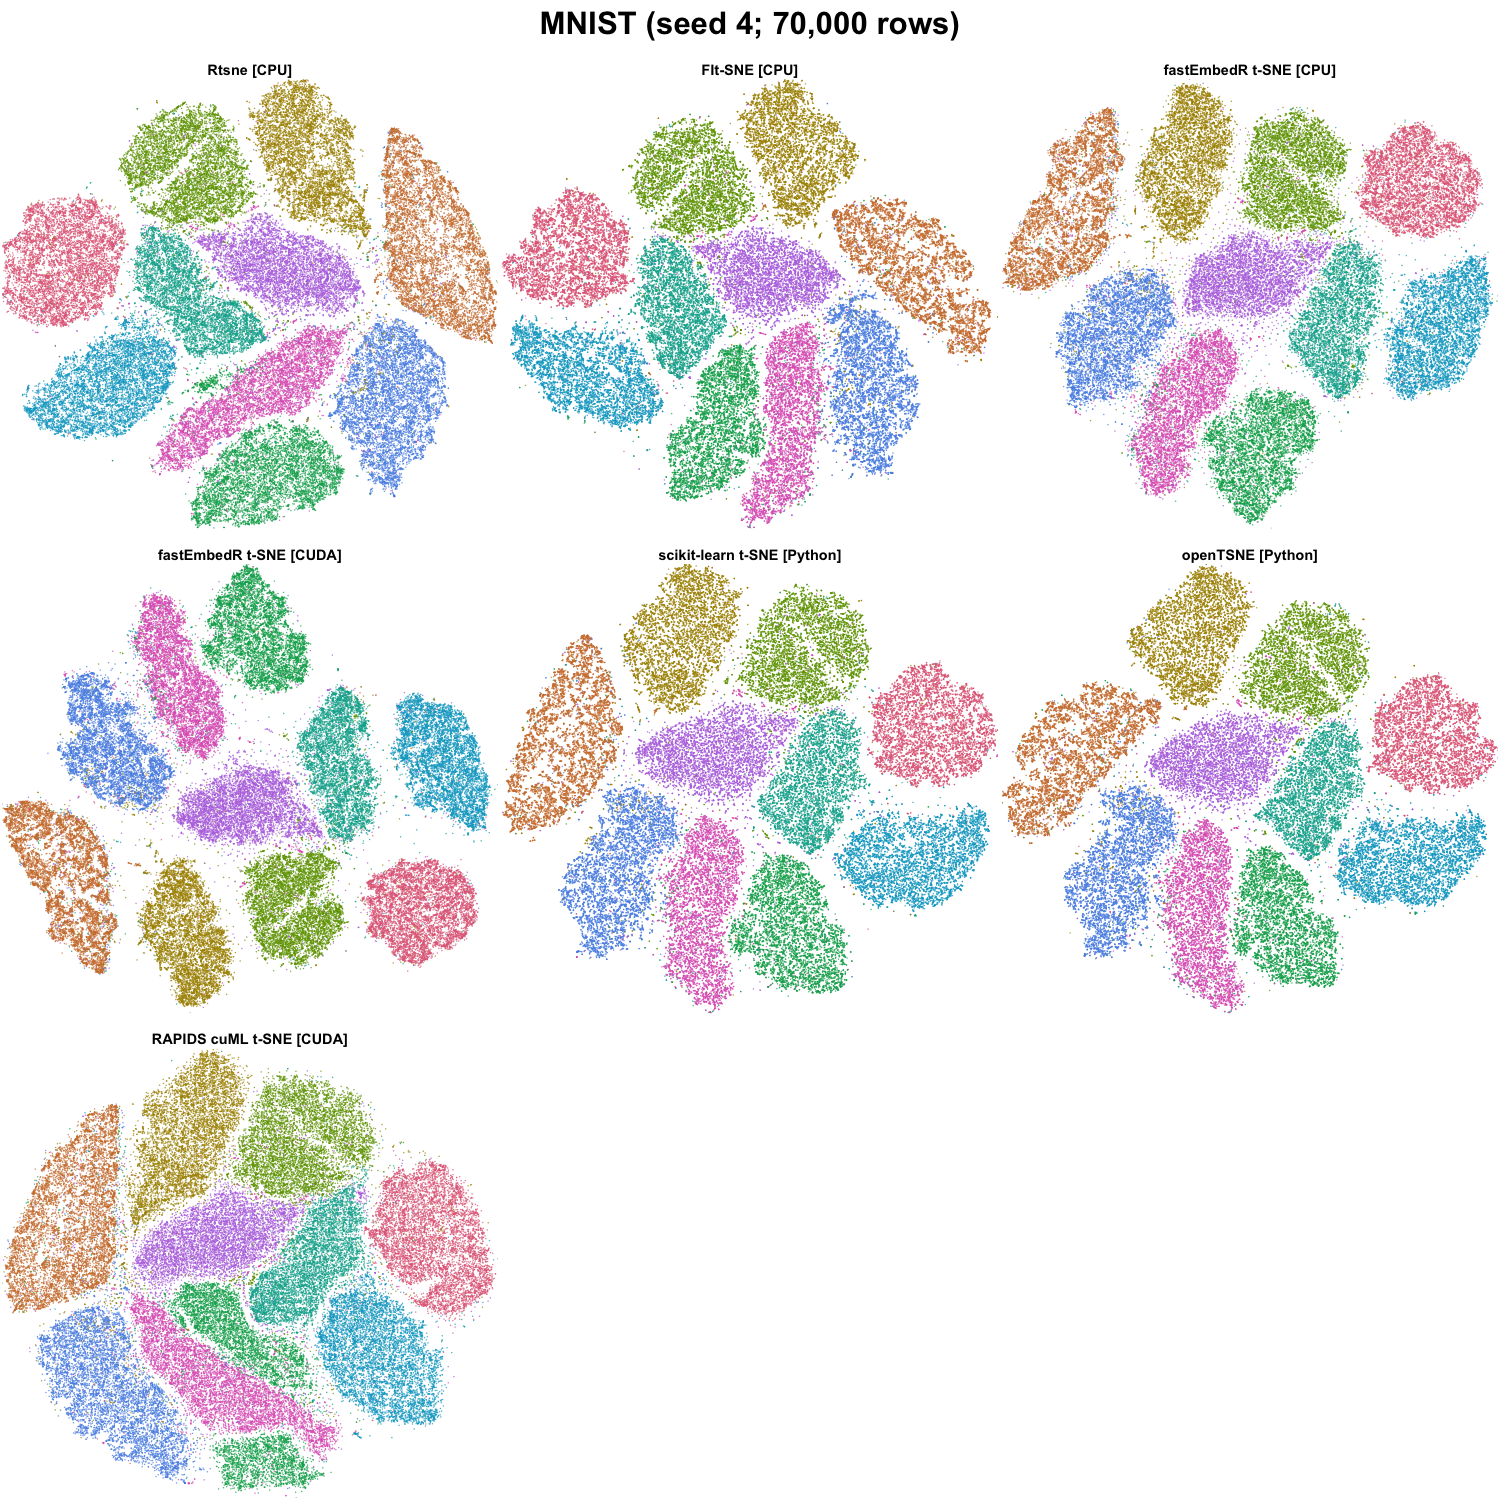
\includegraphics[width=0.94\textwidth]{figures/embedding_all_methods/MNIST_tsne.png}
\caption{MNIST t-SNE outputs for the tested methods (seed 4; 70,000 rows). Colors encode benchmark labels and were not used for fitting.}
\end{figure}
\clearpage

\begin{figure}[p]
\centering
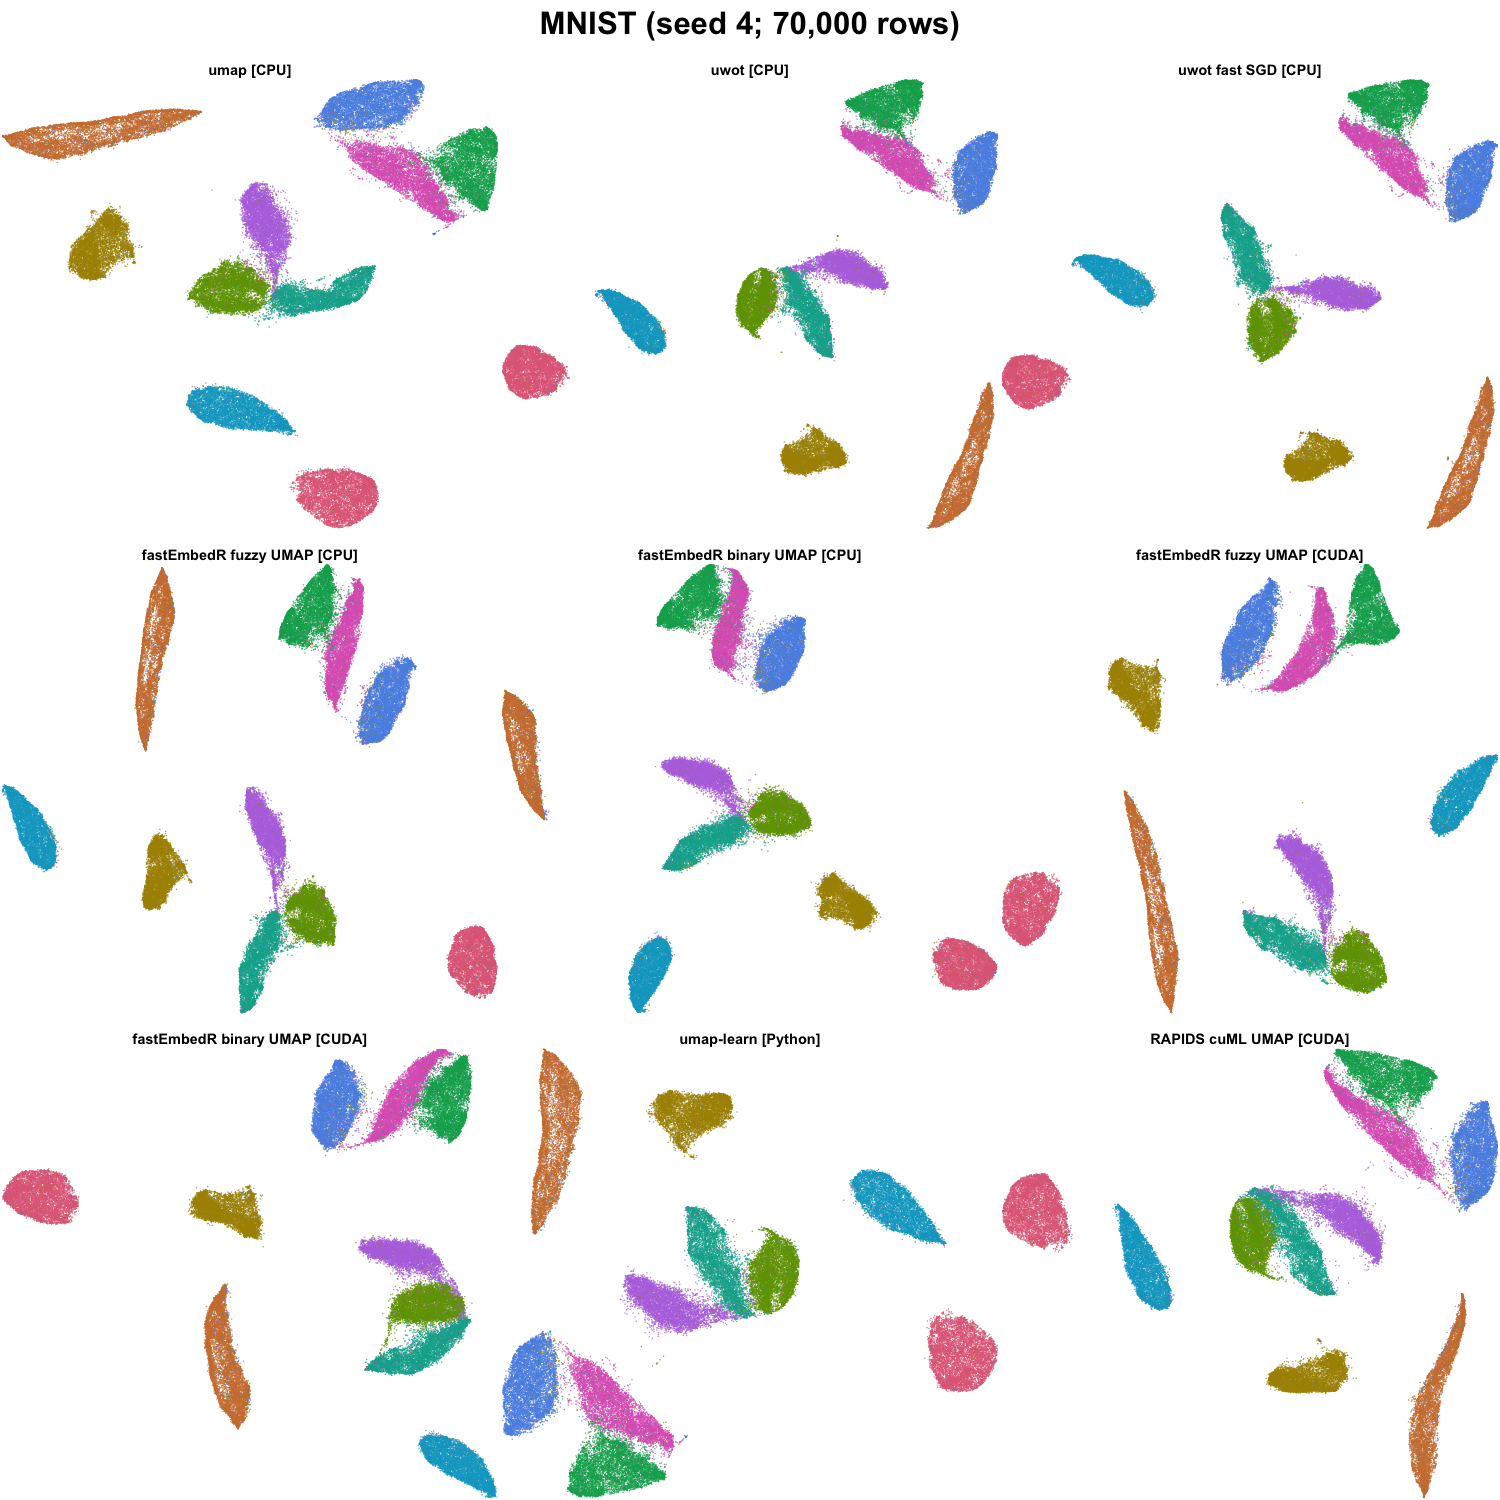
\includegraphics[width=0.94\textwidth]{figures/embedding_all_methods/MNIST_umap.png}
\caption{MNIST UMAP outputs for the tested methods (seed 4; 70,000 rows). Colors encode benchmark labels and were not used for fitting.}
\end{figure}
\clearpage

\begin{figure}[p]
\centering
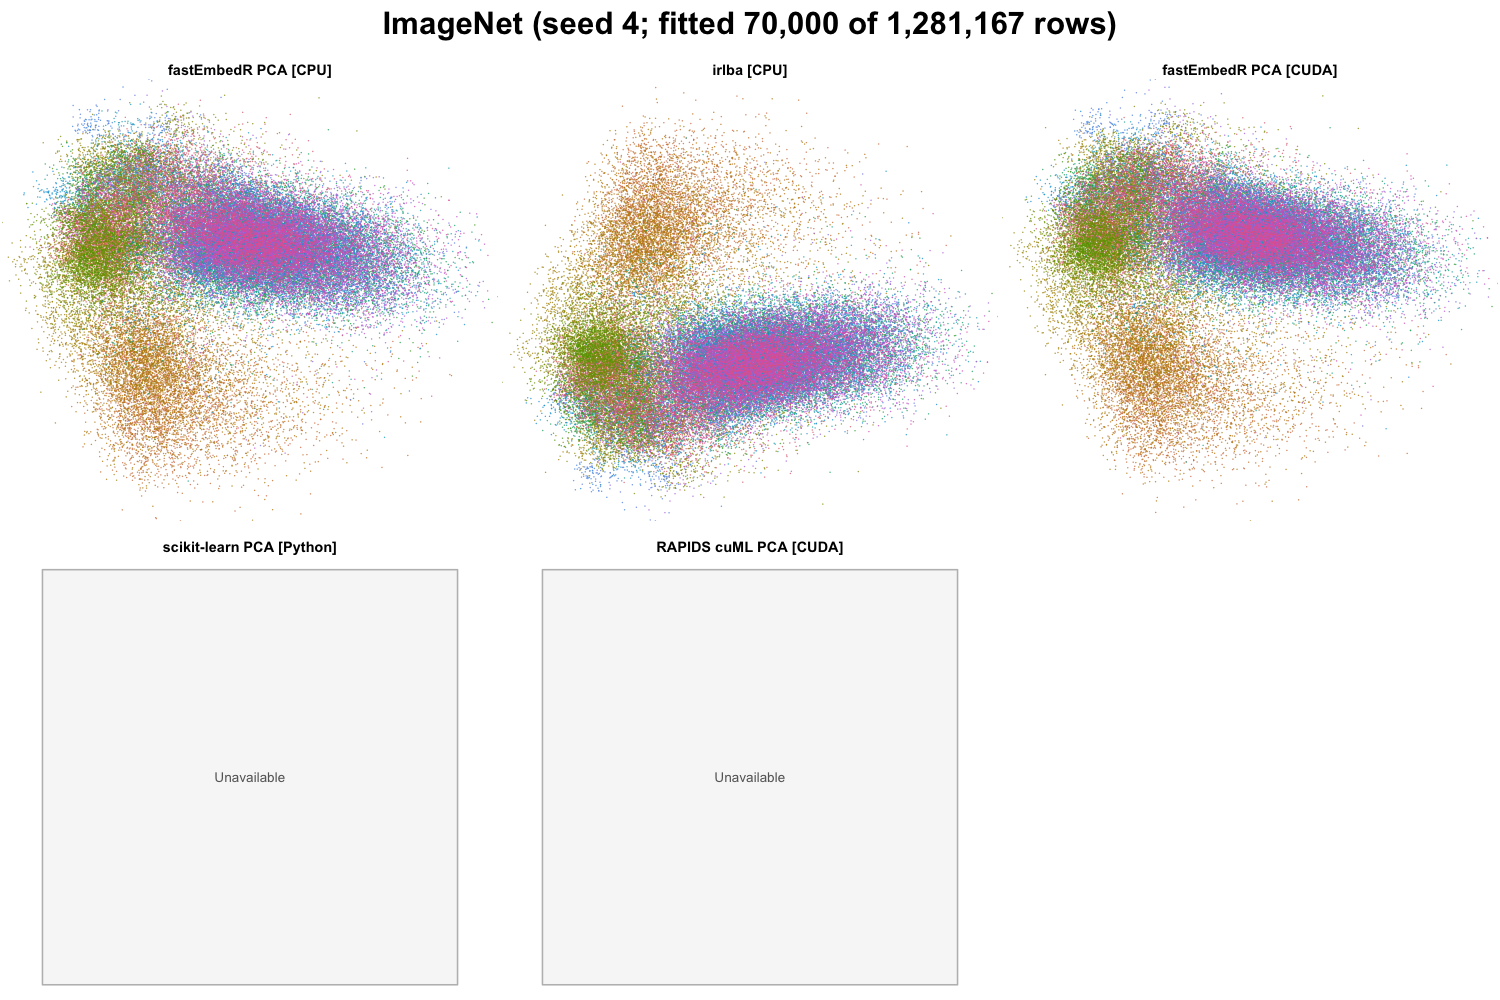
\includegraphics[width=0.94\textwidth]{figures/embedding_all_methods/imagenet_pca.png}
\caption{ImageNet PCA outputs for the tested methods (seed 4; fitted 70,000 of 1,281,167 rows). Colors encode benchmark labels and were not used for fitting.}
\end{figure}
\clearpage

\begin{figure}[p]
\centering
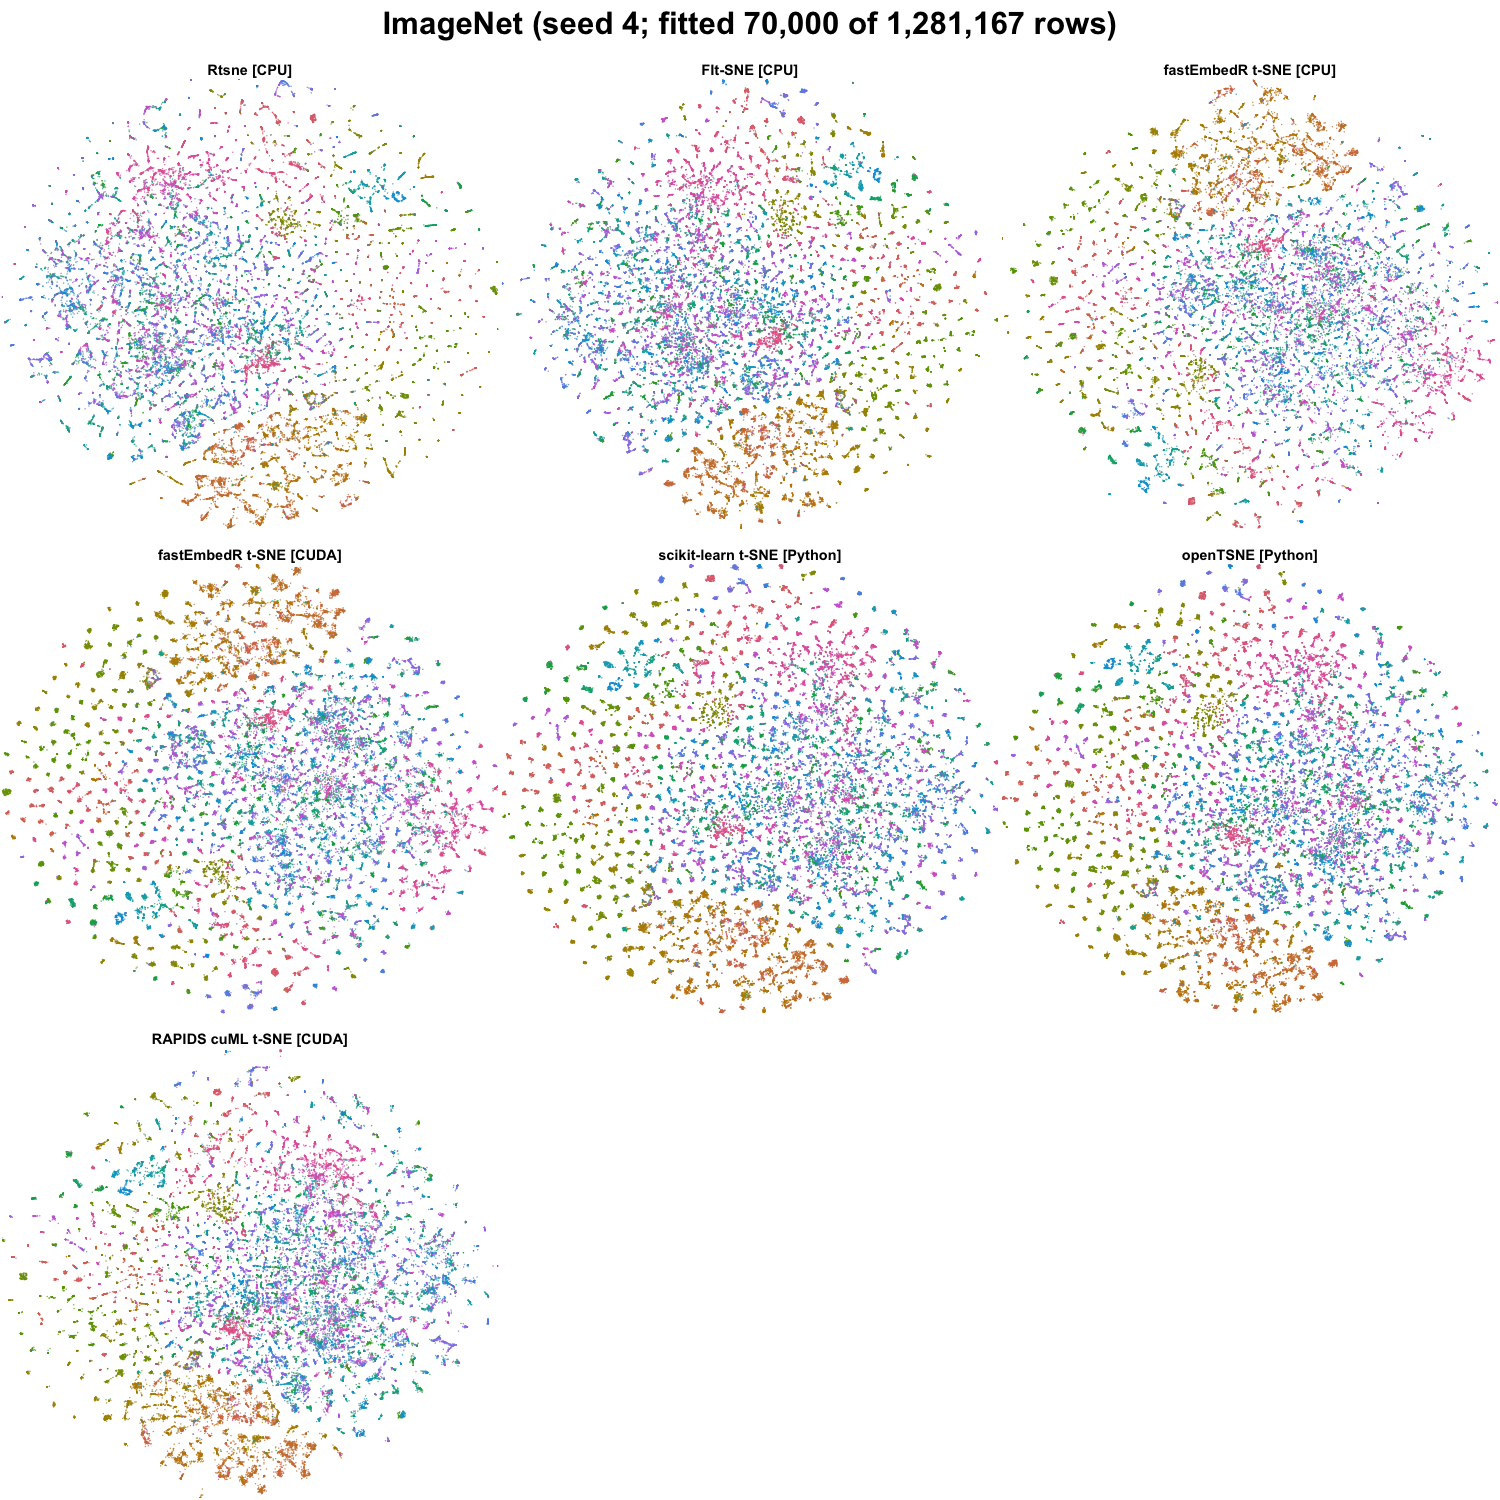
\includegraphics[width=0.94\textwidth]{figures/embedding_all_methods/imagenet_tsne.png}
\caption{ImageNet t-SNE outputs for the tested methods (seed 4; fitted 70,000 of 1,281,167 rows). Colors encode benchmark labels and were not used for fitting.}
\end{figure}
\clearpage

\begin{figure}[p]
\centering
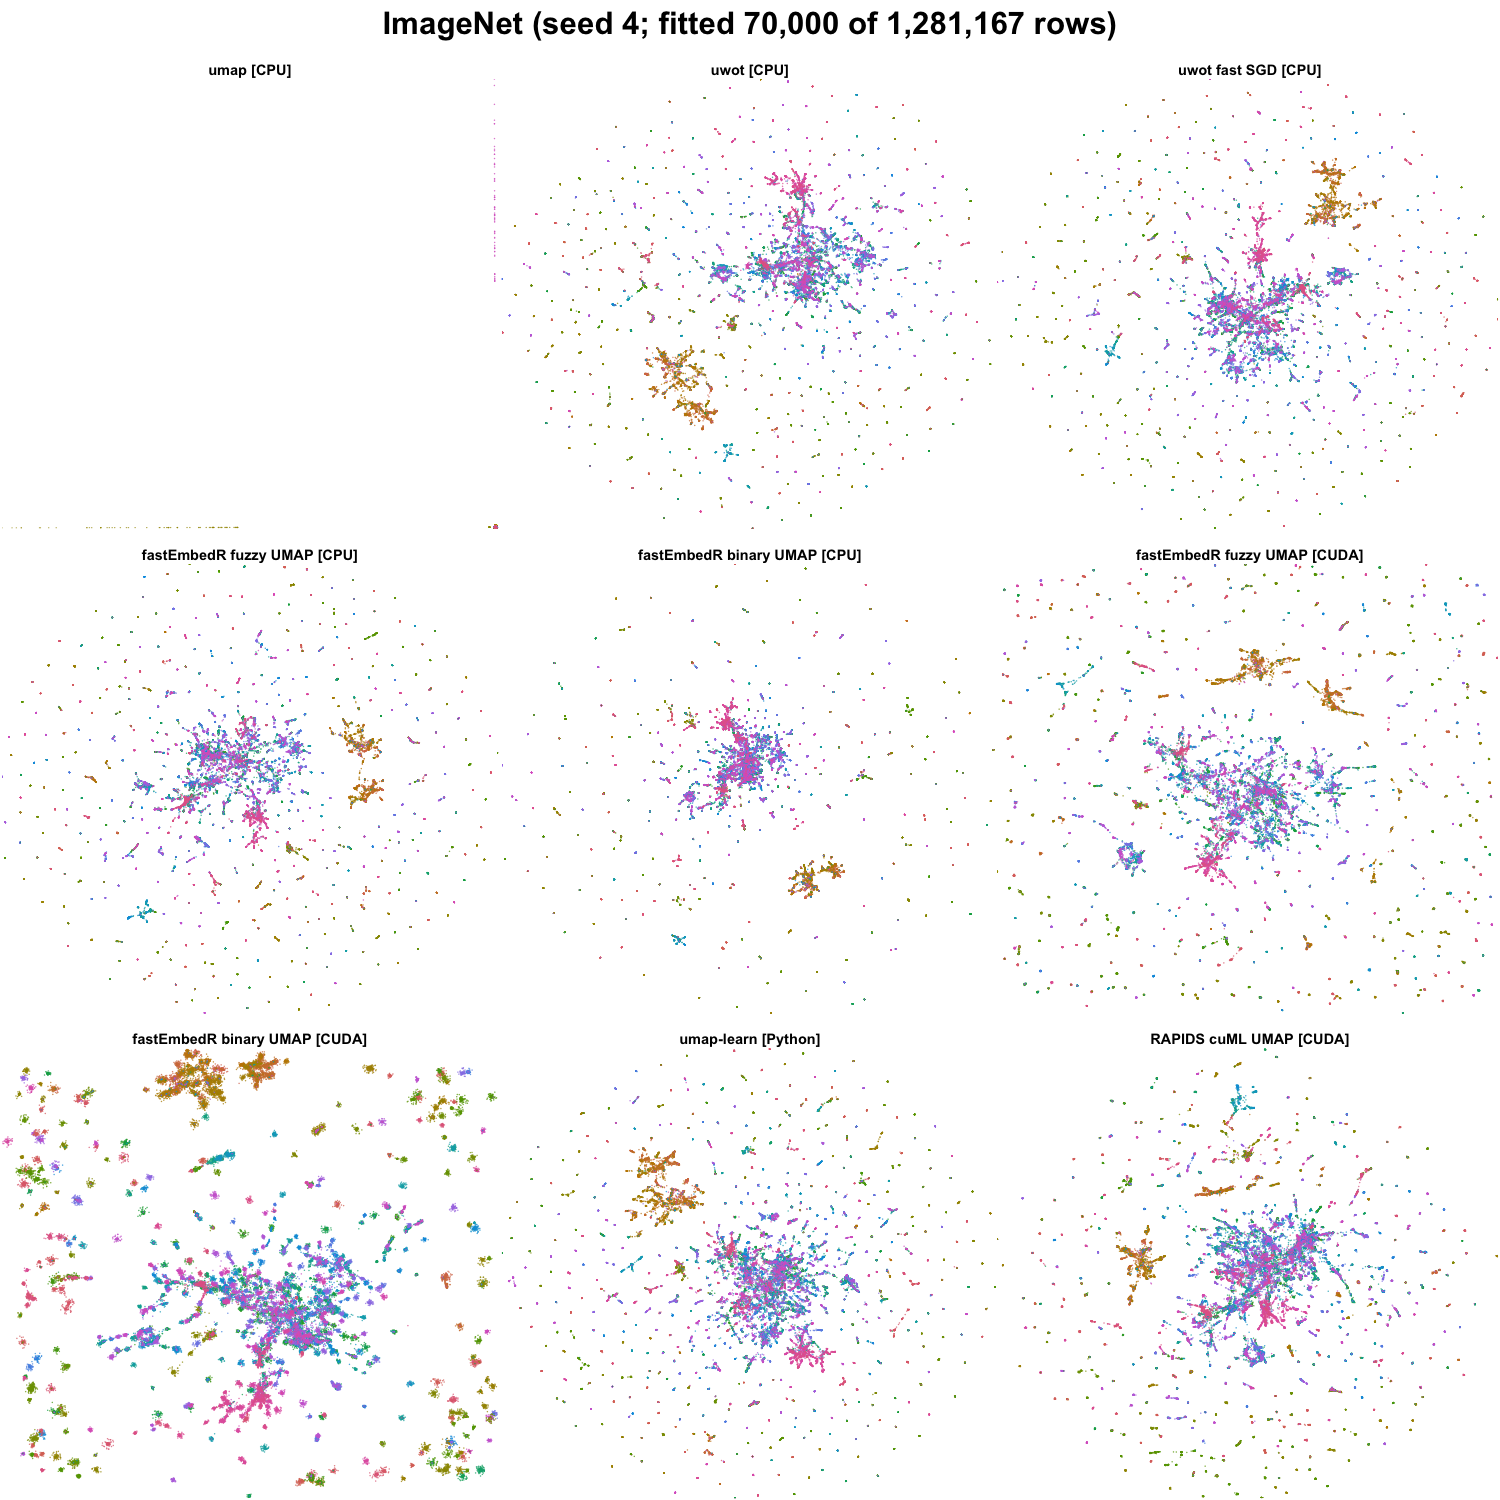
\includegraphics[width=0.94\textwidth]{figures/embedding_all_methods/imagenet_umap.png}
\caption{ImageNet UMAP outputs for the tested methods (seed 4; fitted 70,000 of 1,281,167 rows). Colors encode benchmark labels and were not used for fitting.}
\end{figure}
\clearpage

\begin{figure}[p]
\centering
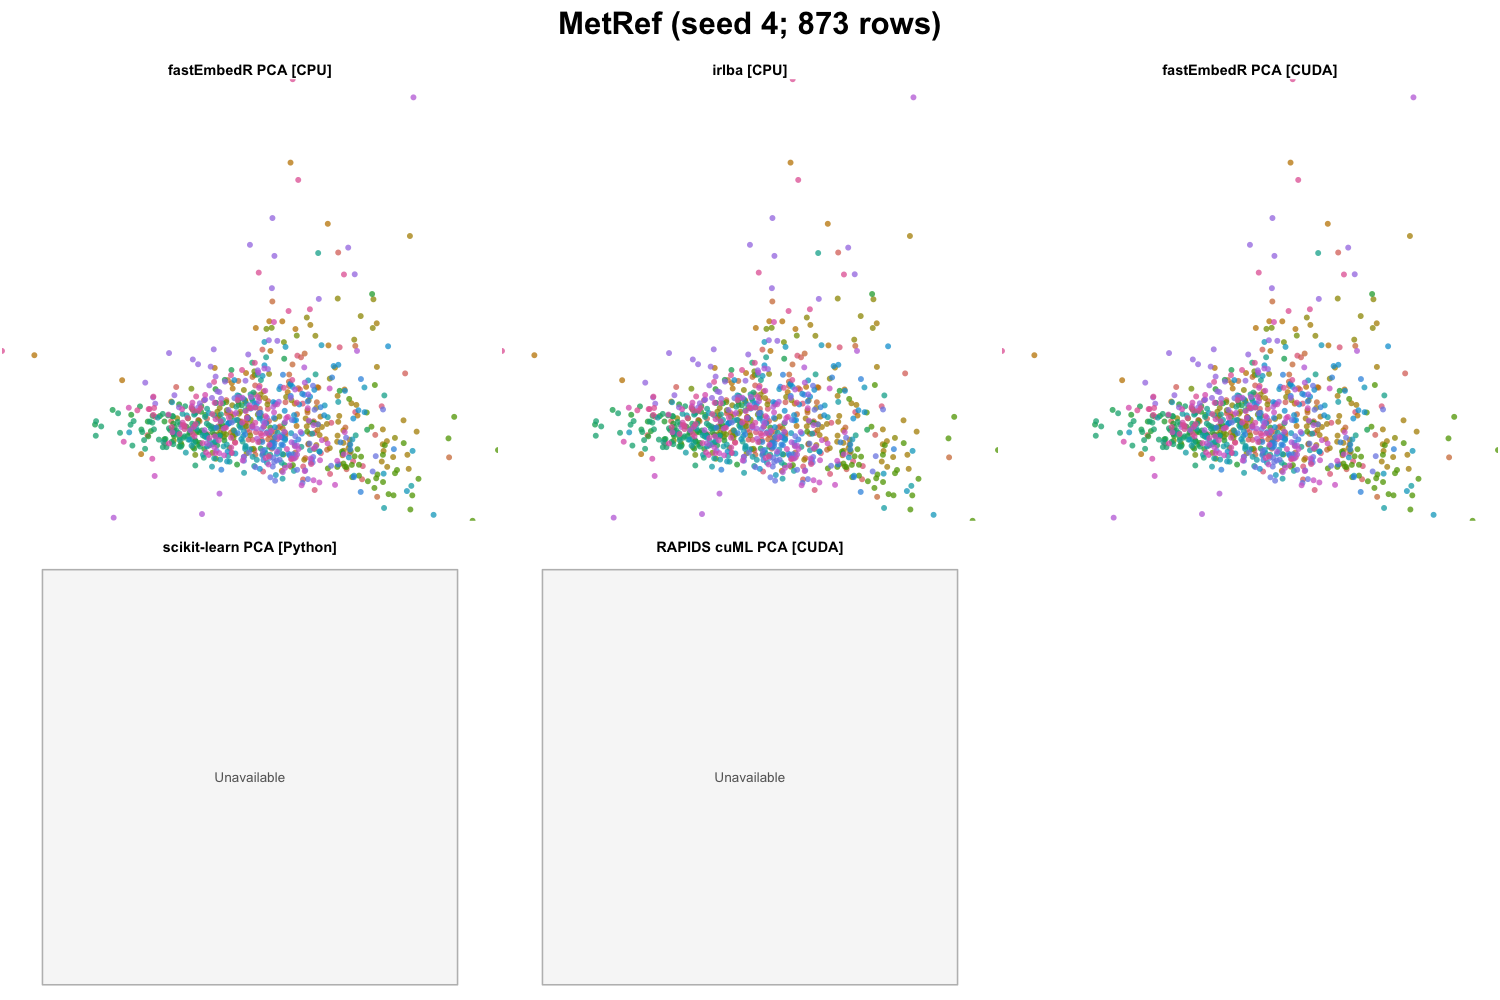
\includegraphics[width=0.94\textwidth]{figures/embedding_all_methods/MetRef_pca.png}
\caption{MetRef PCA outputs for the tested methods (seed 4; 873 rows). Colors encode benchmark labels and were not used for fitting.}
\end{figure}
\clearpage

\begin{figure}[p]
\centering
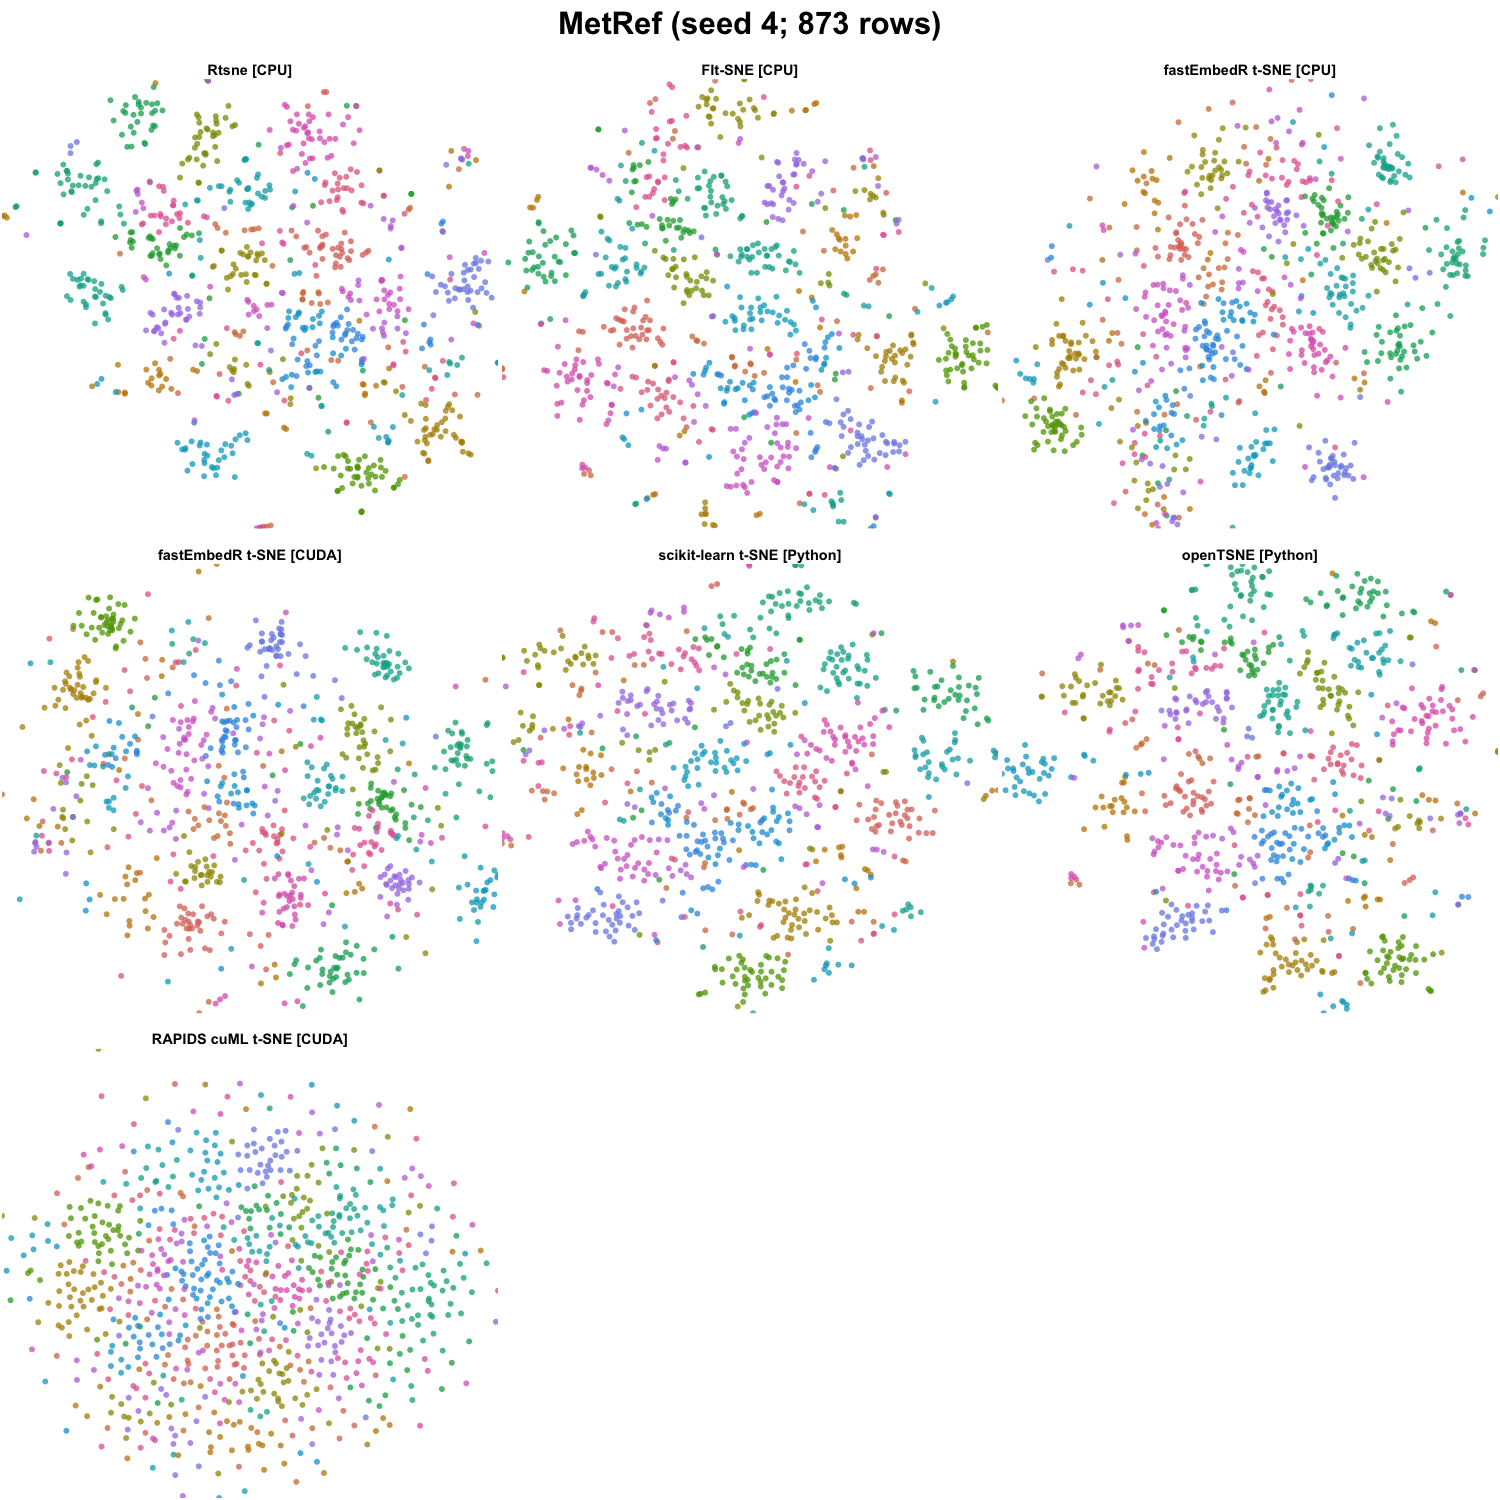
\includegraphics[width=0.94\textwidth]{figures/embedding_all_methods/MetRef_tsne.png}
\caption{MetRef t-SNE outputs for the tested methods (seed 4; 873 rows). Colors encode benchmark labels and were not used for fitting.}
\end{figure}
\clearpage

\begin{figure}[p]
\centering
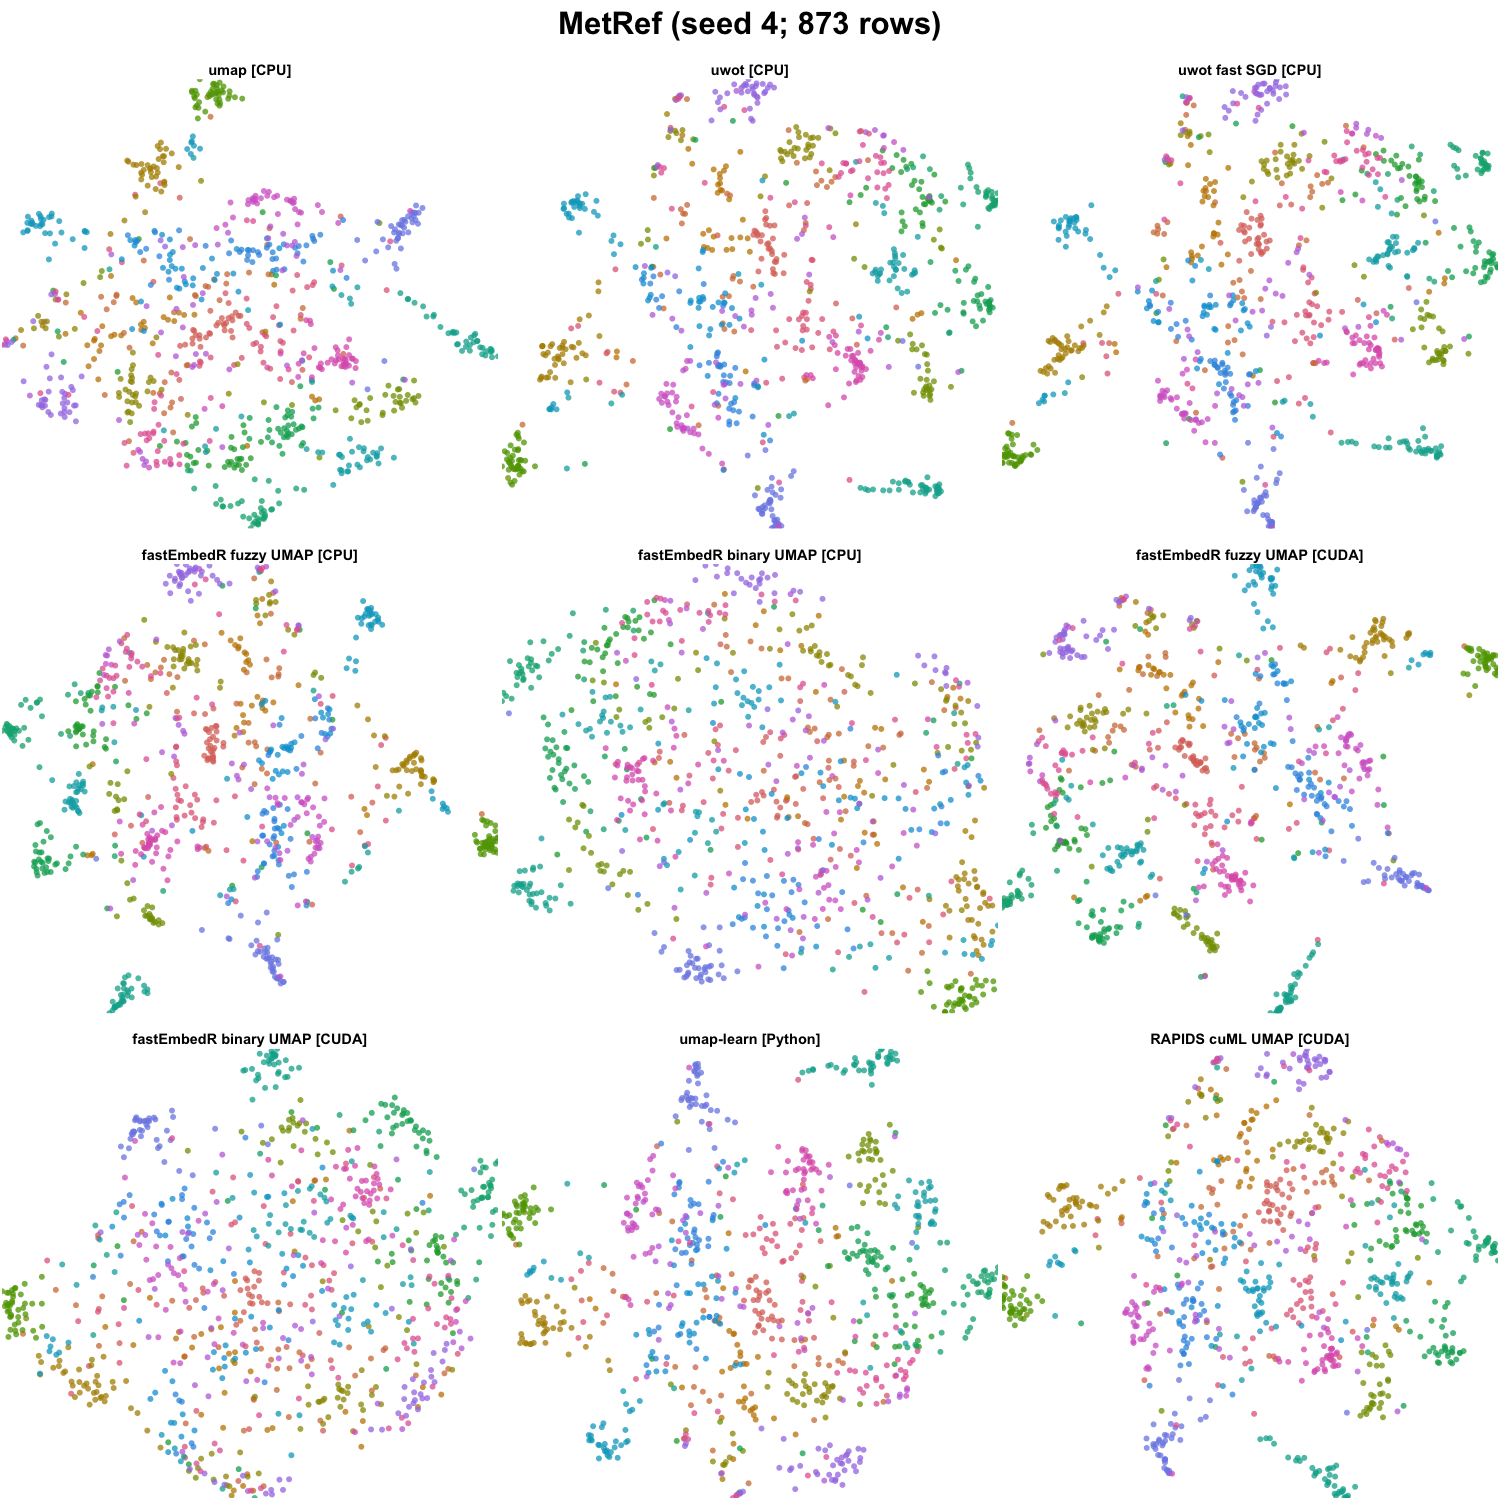
\includegraphics[width=0.94\textwidth]{figures/embedding_all_methods/MetRef_umap.png}
\caption{MetRef UMAP outputs for the tested methods (seed 4; 873 rows). Colors encode benchmark labels and were not used for fitting.}
\end{figure}
\clearpage

\begin{figure}[p]
\centering
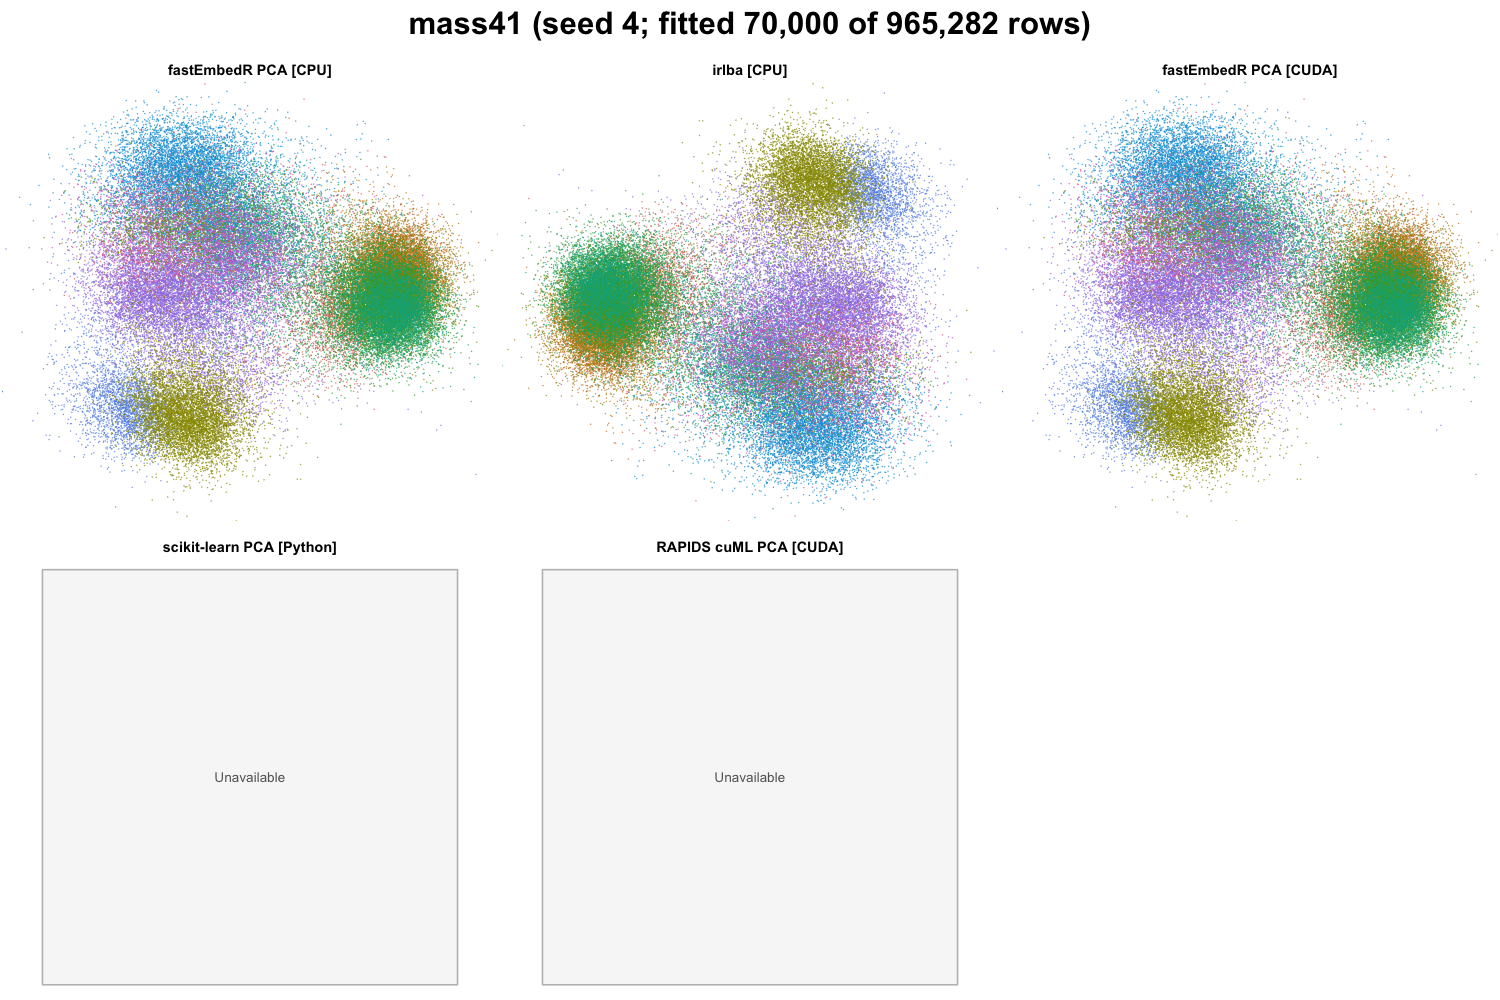
\includegraphics[width=0.94\textwidth]{figures/embedding_all_methods/mass41_pca.png}
\caption{mass41 PCA outputs for the tested methods (seed 4; fitted 70,000 of 965,282 rows). Colors encode benchmark labels and were not used for fitting.}
\end{figure}
\clearpage

\begin{figure}[p]
\centering
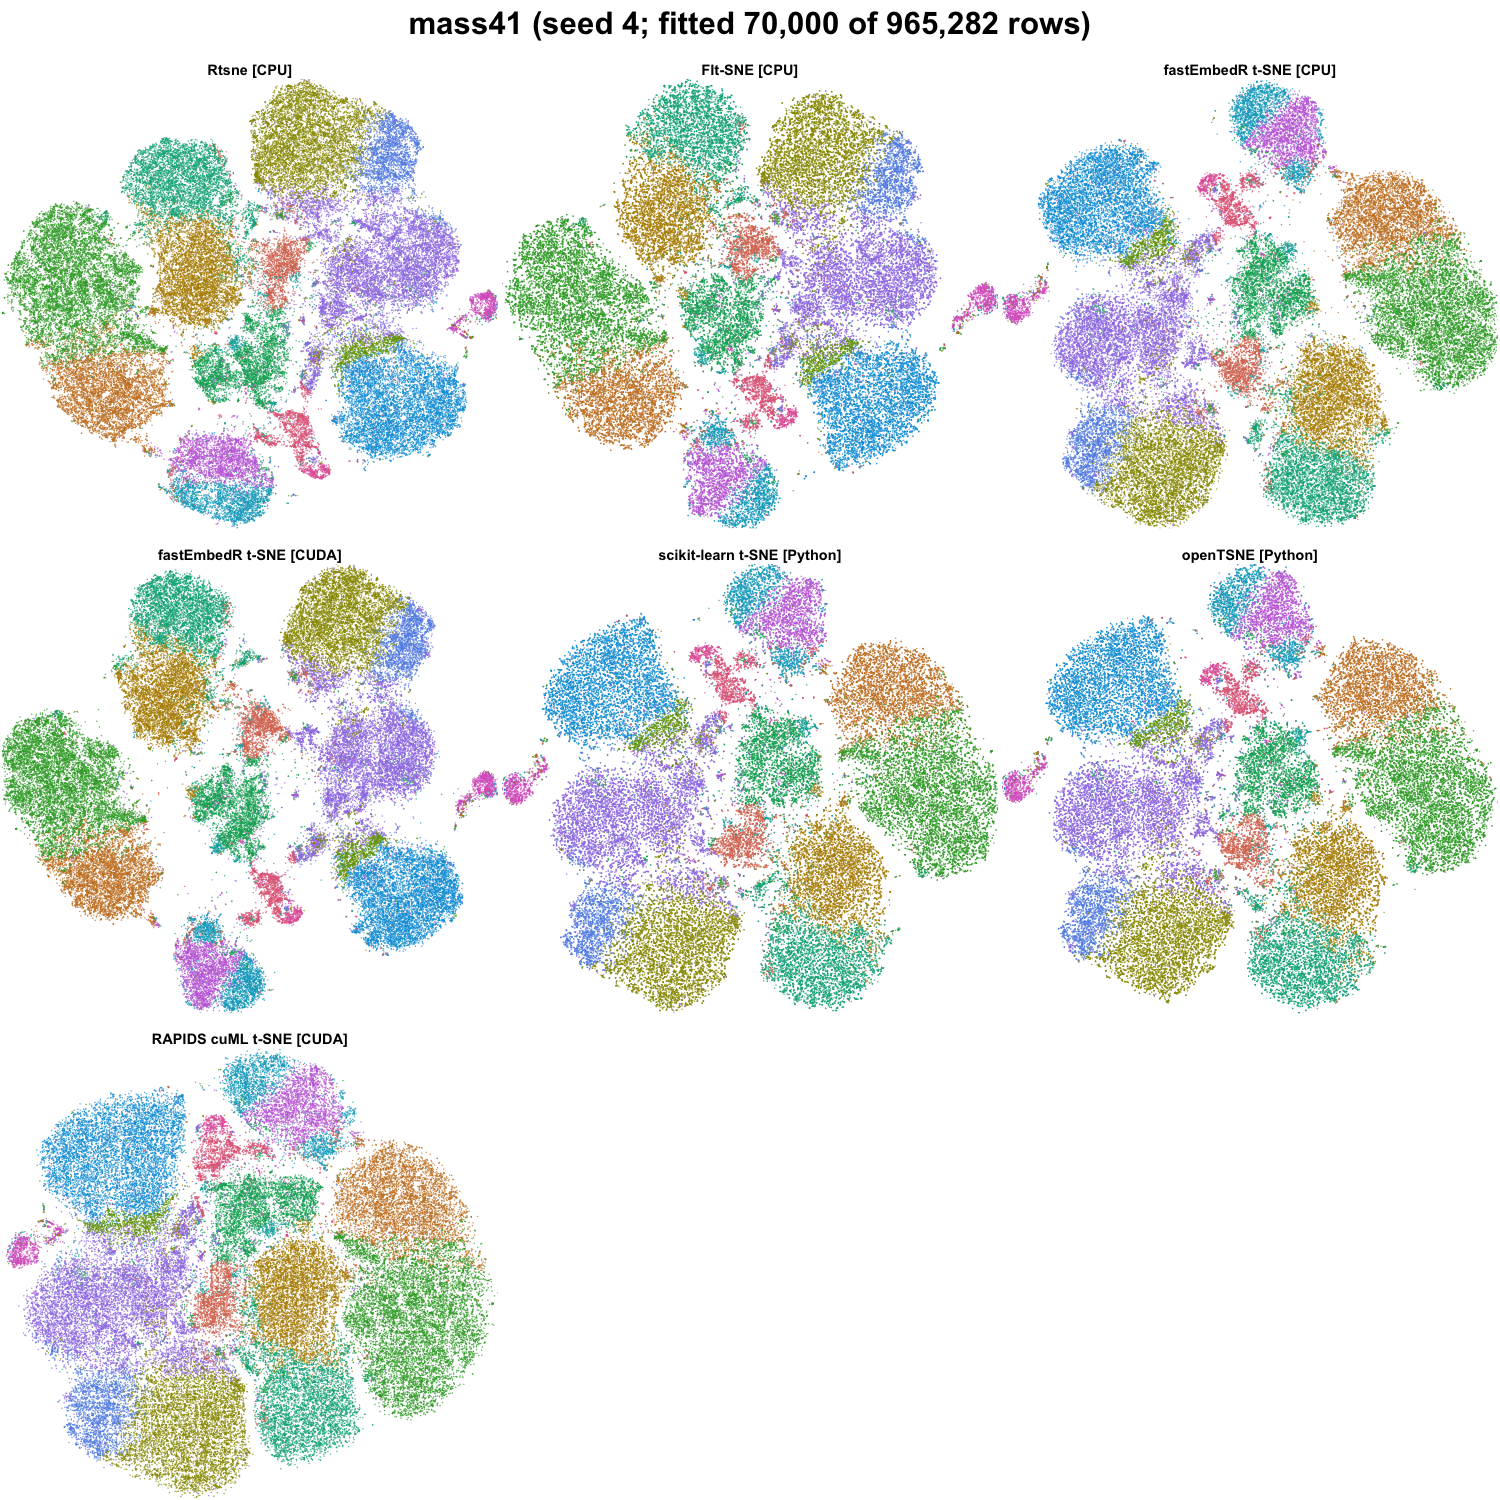
\includegraphics[width=0.94\textwidth]{figures/embedding_all_methods/mass41_tsne.png}
\caption{mass41 t-SNE outputs for the tested methods (seed 4; fitted 70,000 of 965,282 rows). Colors encode benchmark labels and were not used for fitting.}
\end{figure}
\clearpage

\begin{figure}[p]
\centering
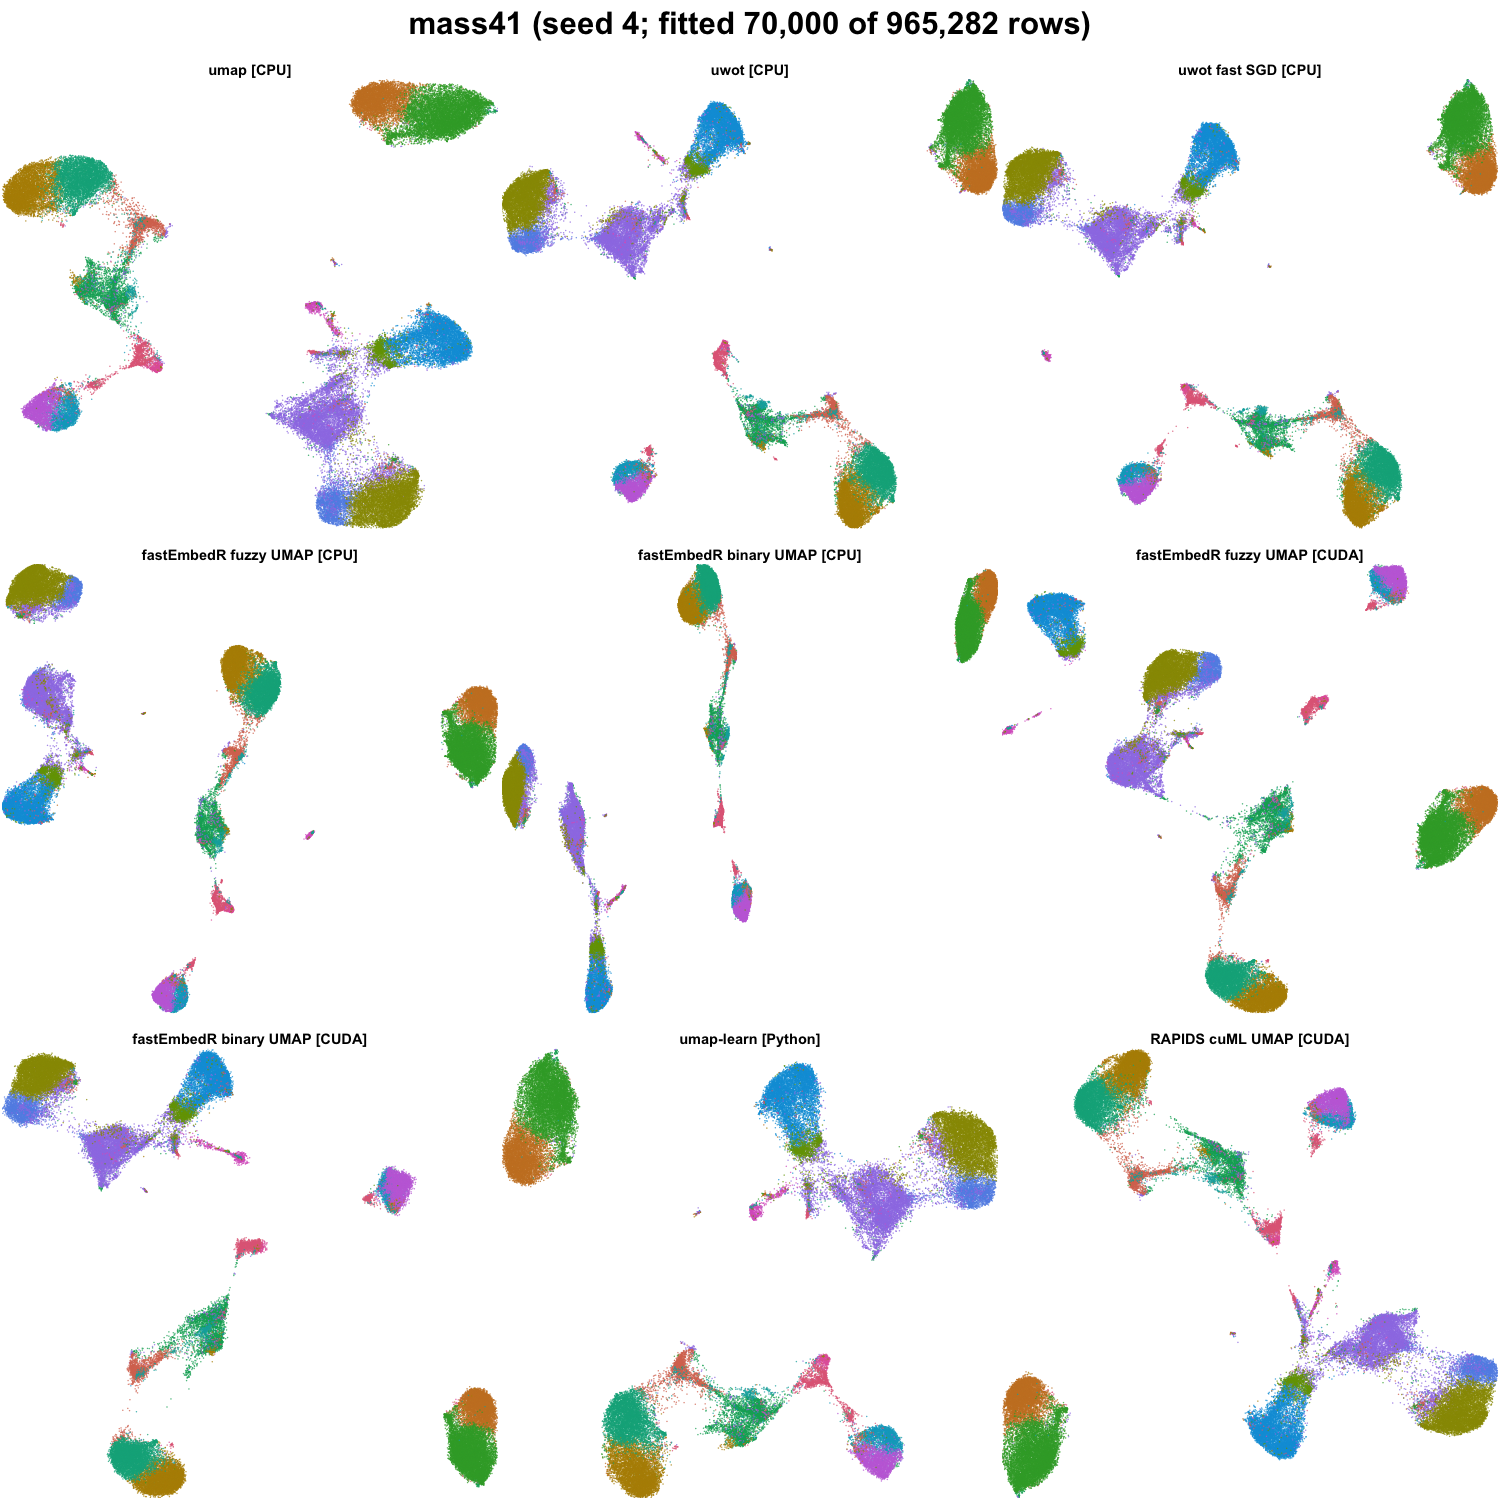
\includegraphics[width=0.94\textwidth]{figures/embedding_all_methods/mass41_umap.png}
\caption{mass41 UMAP outputs for the tested methods (seed 4; fitted 70,000 of 965,282 rows). Colors encode benchmark labels and were not used for fitting.}
\end{figure}
\clearpage

\begin{figure}[p]
\centering
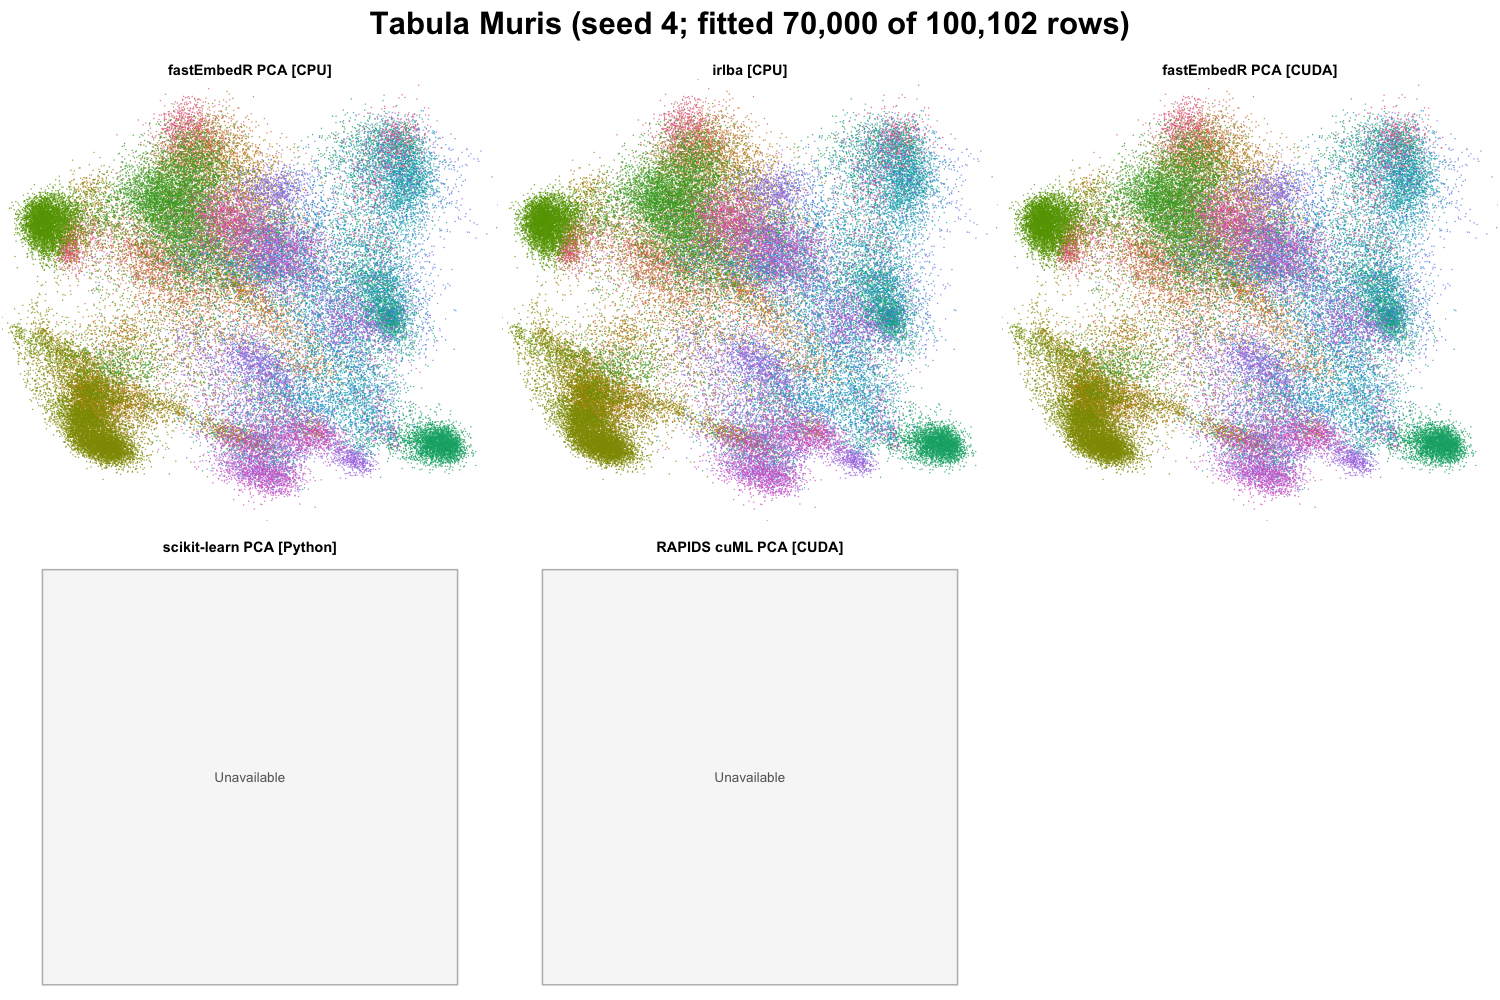
\includegraphics[width=0.94\textwidth]{figures/embedding_all_methods/TabulaMuris_pca.png}
\caption{Tabula Muris PCA outputs for the tested methods (seed 4; fitted 70,000 of 100,102 rows). Colors encode benchmark labels and were not used for fitting.}
\end{figure}
\clearpage

\begin{figure}[p]
\centering
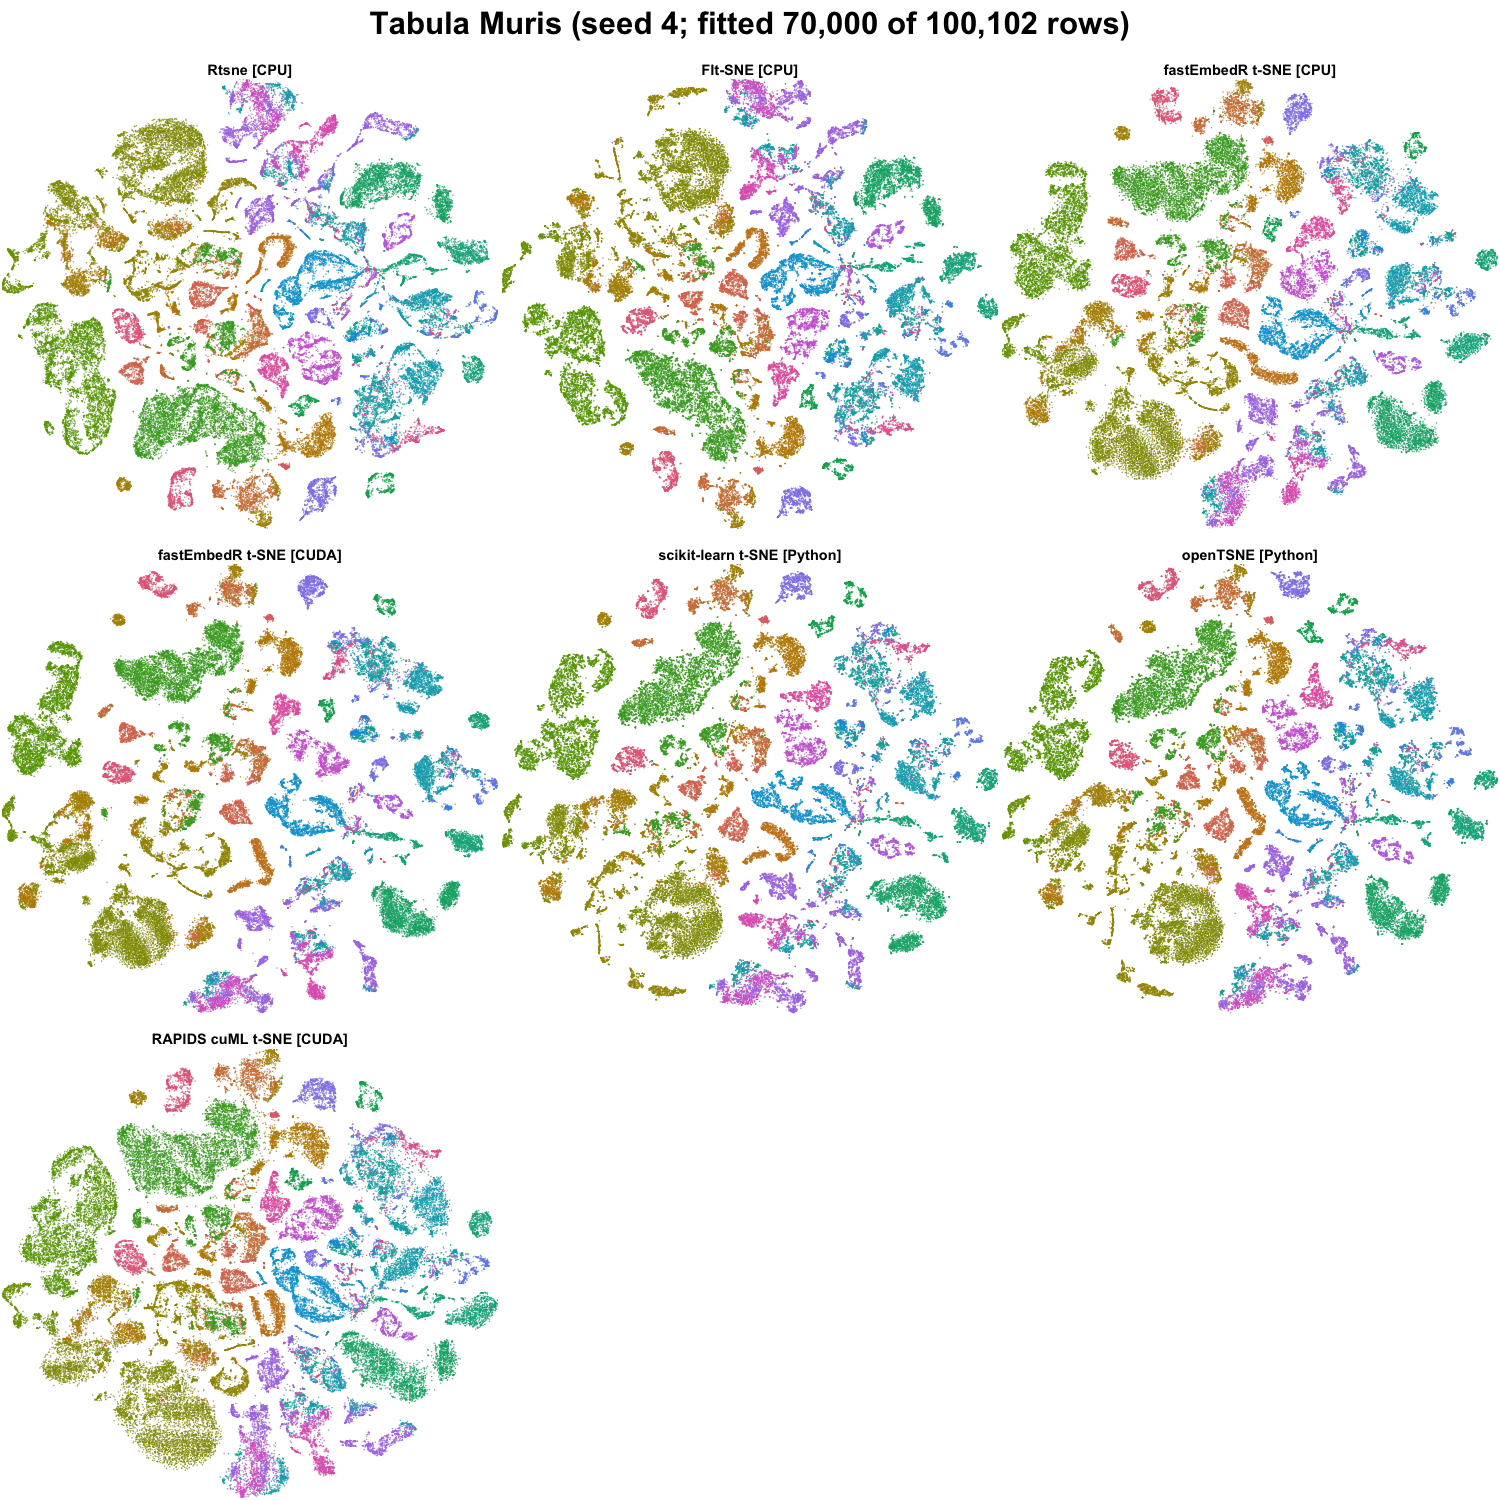
\includegraphics[width=0.94\textwidth]{figures/embedding_all_methods/TabulaMuris_tsne.png}
\caption{Tabula Muris t-SNE outputs for the tested methods (seed 4; fitted 70,000 of 100,102 rows). Colors encode benchmark labels and were not used for fitting.}
\end{figure}
\clearpage

\begin{figure}[p]
\centering
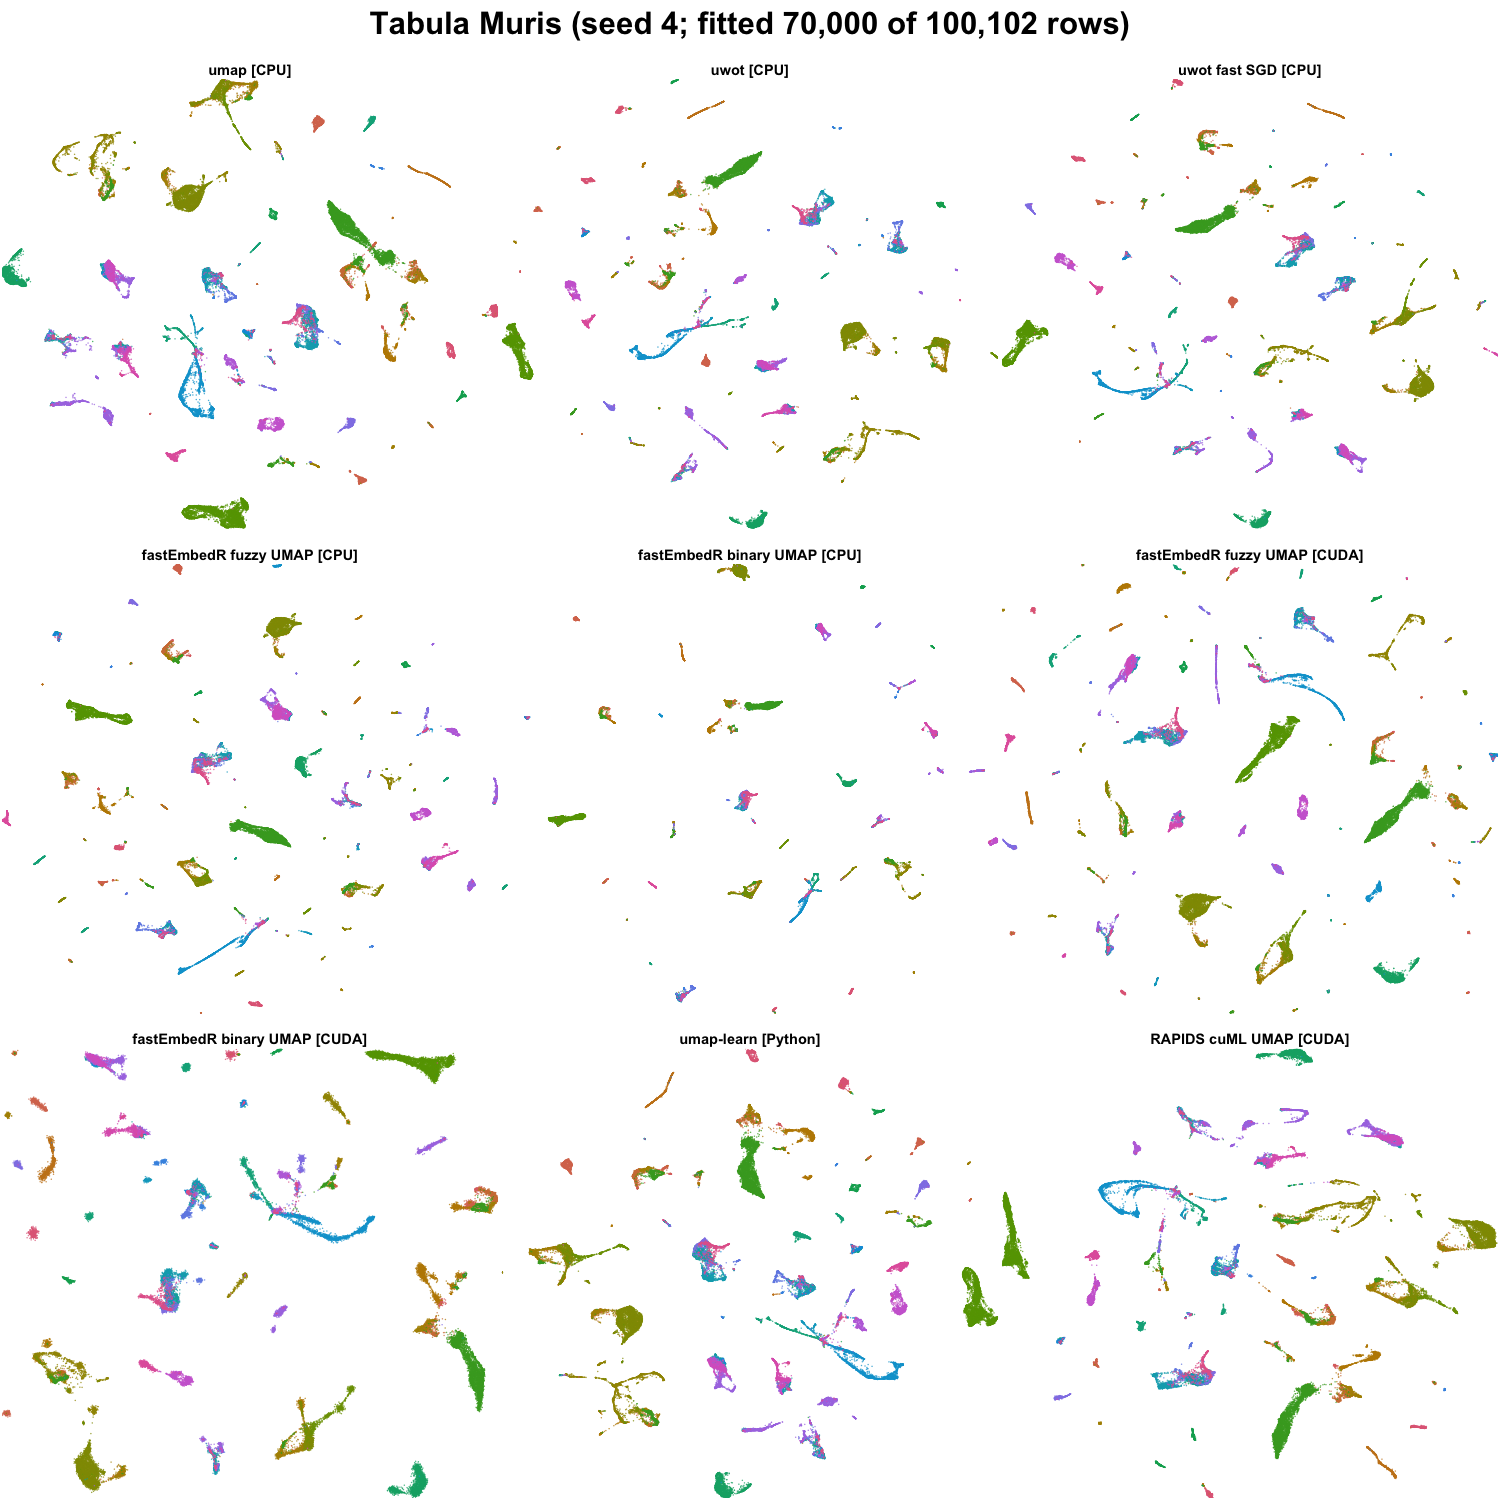
\includegraphics[width=0.94\textwidth]{figures/embedding_all_methods/TabulaMuris_umap.png}
\caption{Tabula Muris UMAP outputs for the tested methods (seed 4; fitted 70,000 of 100,102 rows). Colors encode benchmark labels and were not used for fitting.}
\end{figure}
\clearpage

\begin{figure}[p]
\centering
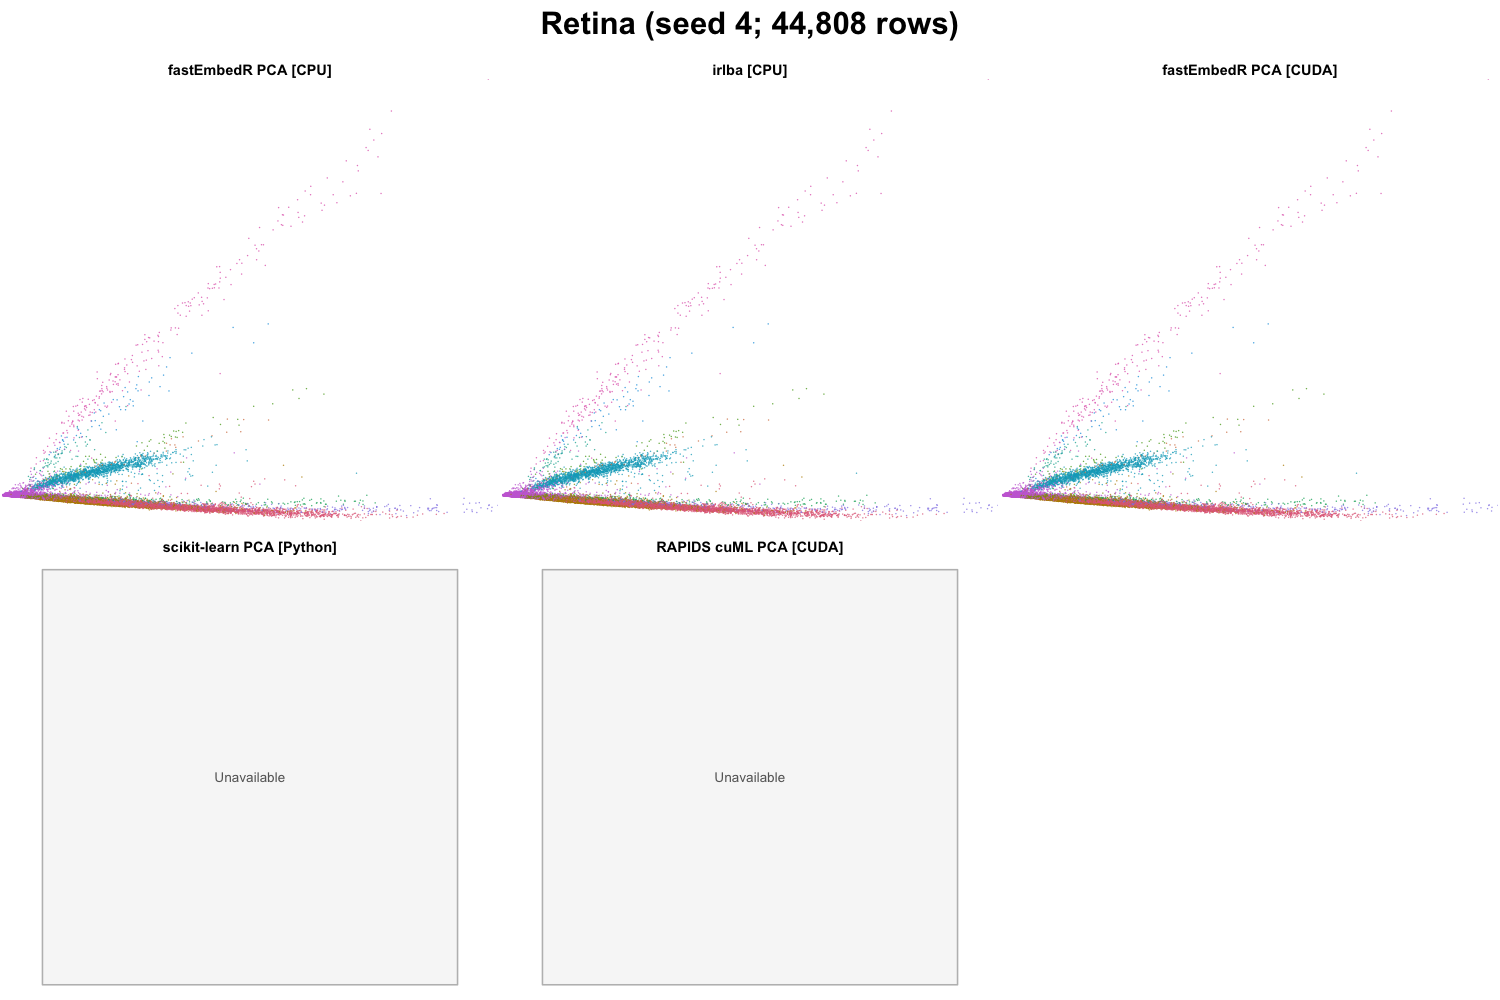
\includegraphics[width=0.94\textwidth]{figures/embedding_all_methods/Macosko2015_retina_pca.png}
\caption{Retina PCA outputs for the tested methods (seed 4; 44,808 rows). Colors encode benchmark labels and were not used for fitting.}
\end{figure}
\clearpage

\begin{figure}[p]
\centering
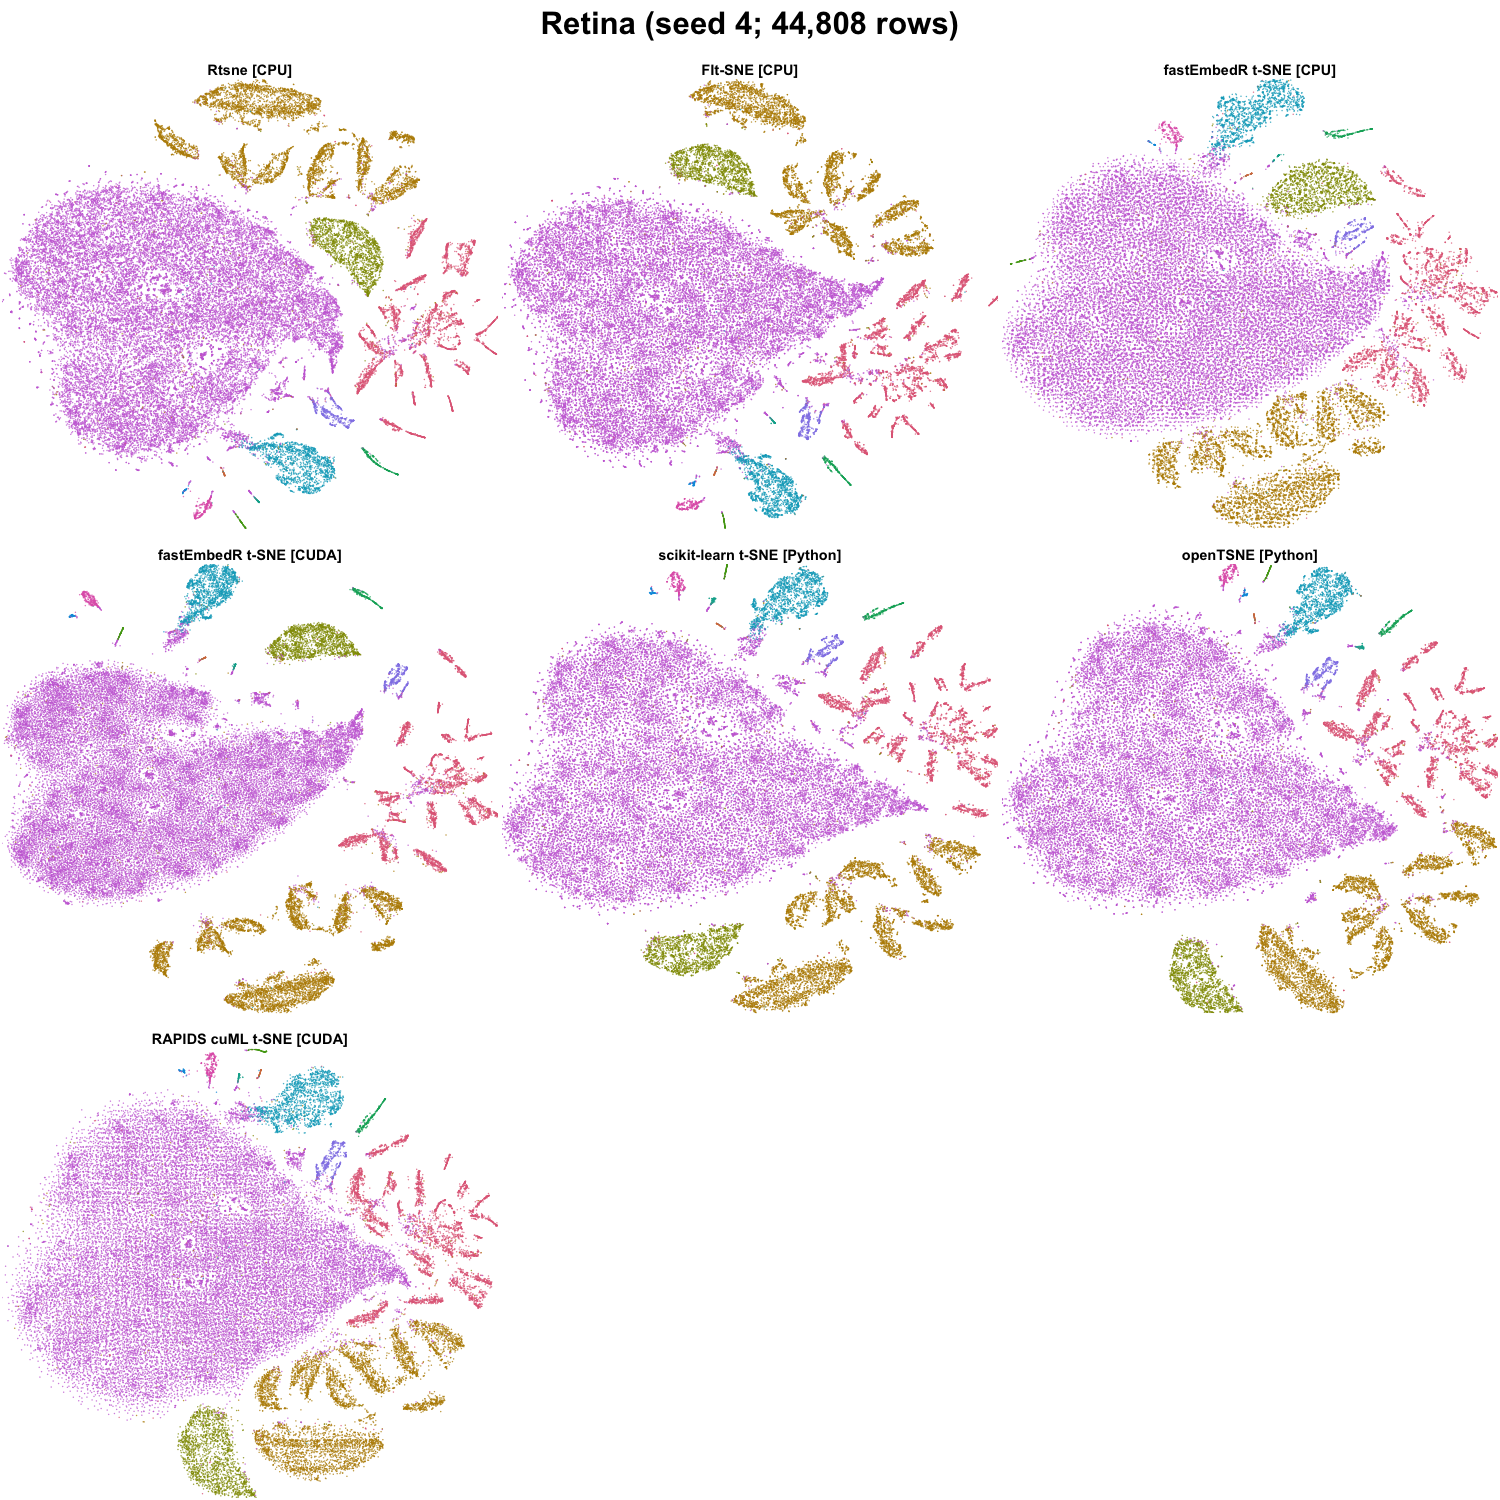
\includegraphics[width=0.94\textwidth]{figures/embedding_all_methods/Macosko2015_retina_tsne.png}
\caption{Retina t-SNE outputs for the tested methods (seed 4; 44,808 rows). Colors encode benchmark labels and were not used for fitting.}
\end{figure}
\clearpage

\begin{figure}[p]
\centering
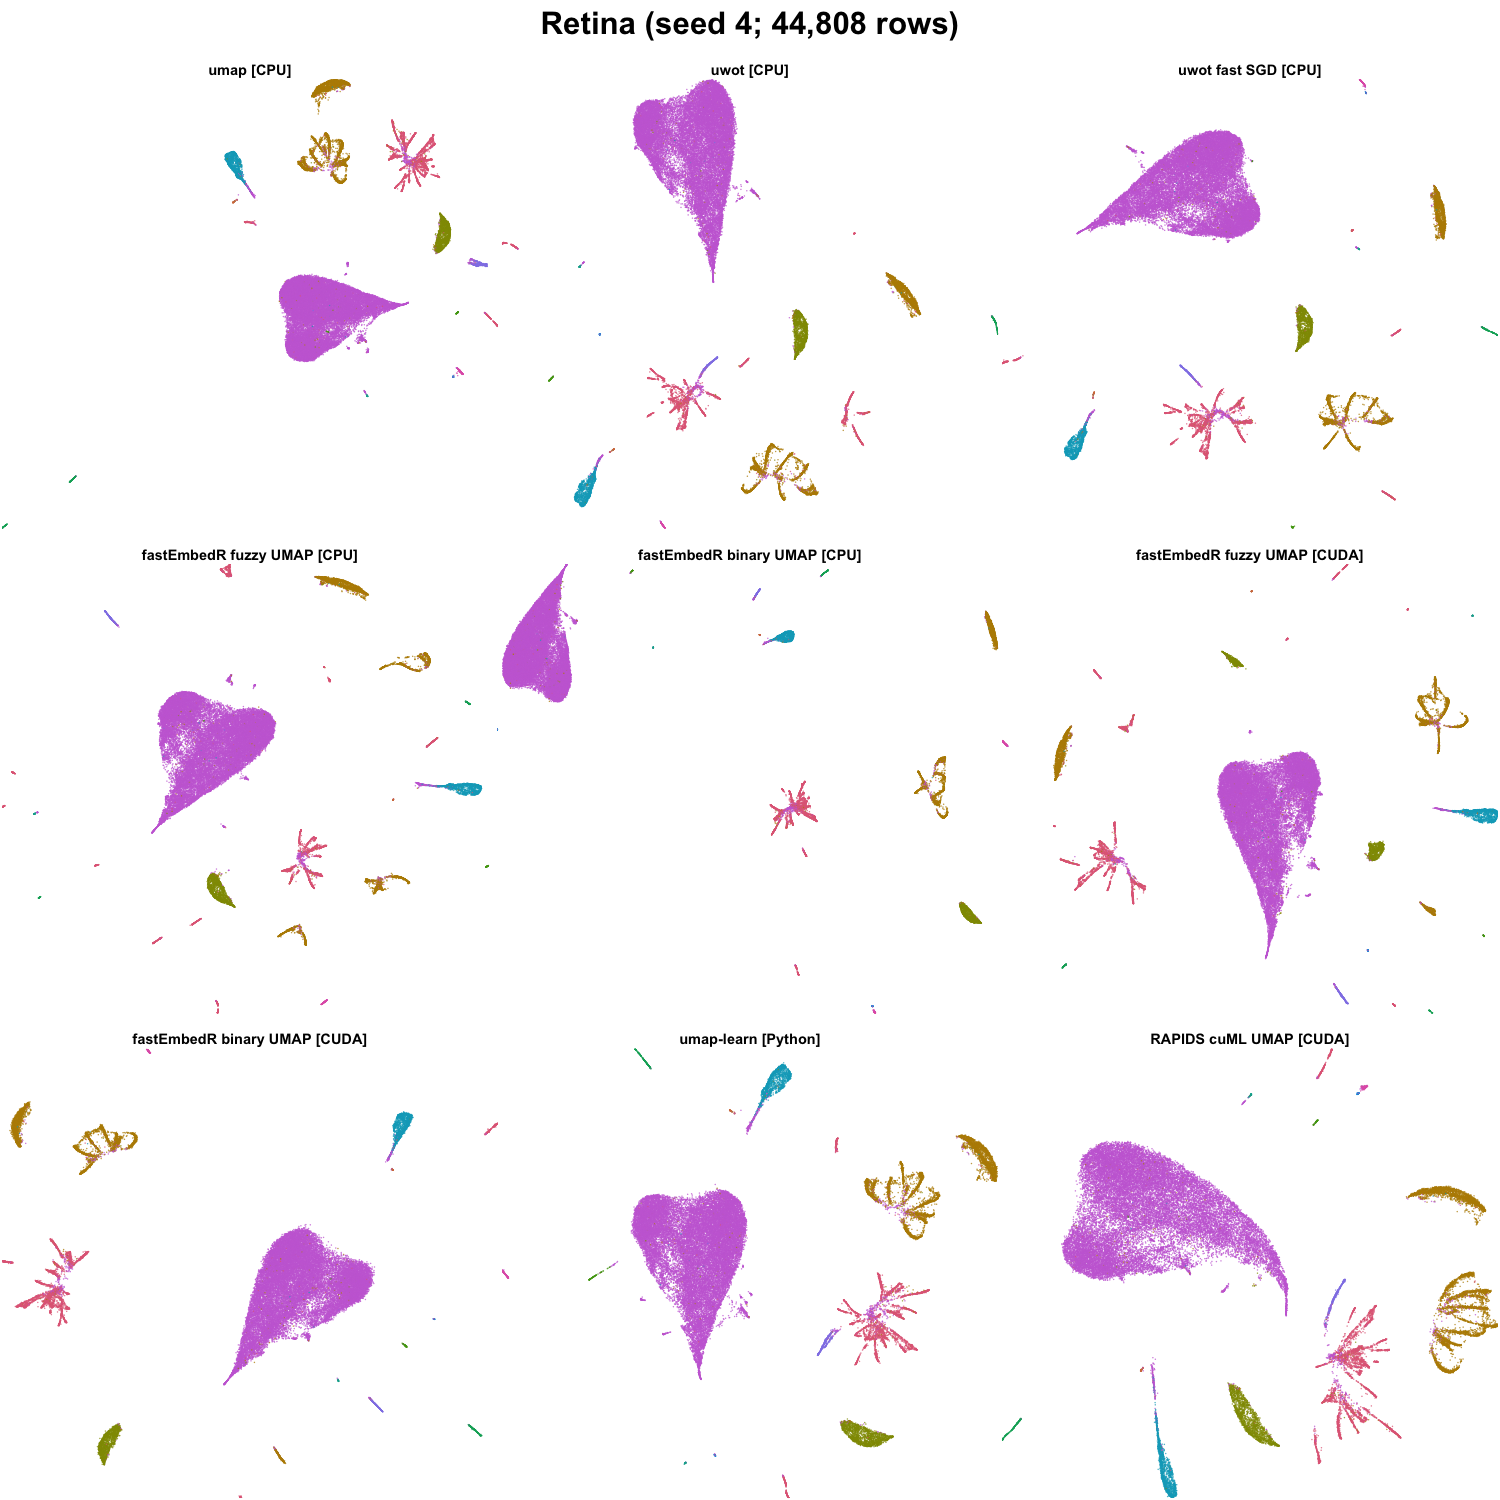
\includegraphics[width=0.94\textwidth]{figures/embedding_all_methods/Macosko2015_retina_umap.png}
\caption{Retina UMAP outputs for the tested methods (seed 4; 44,808 rows). Colors encode benchmark labels and were not used for fitting.}
\end{figure}
\clearpage
